\documentclass{particles2015}

\usepackage{graphicx}
\usepackage{amsmath}
\usepackage{amsfonts}
\usepackage{amssymb}
\usepackage{epstopdf}
%\usepackage{subfigure}
%\usepackage{subcaption}
\usepackage{caption}
\usepackage{subcaption}

\title{DEM particle characterization by artificial neural networks and macroscopic experiments}

\author{Luca~BENVENUTI $^{1}$, Christoph~KLOSS $^{2}$, Stefan~PIRKER $^{1}$}

\heading{Luca~Benvenuti, Christoph~Kloss, Stefan~Pirker}

\address{$^{1}$ Johannes Kepler University Linz, Department on Particulate Flow
Mode lling\\
Altenbergerstrasse 69, 4040, Linz, Austria \\
luca.benvenuti@jku.at - www.jku.at/pfm
\and
$^{3}$ DCS Computing GmbH\\
Altenbergerstr. 66a - Science Park, 4040 Linz, Austria \\
christoph.kloss@dcs-computing.com - www.dcs-computing.com}

\keywords{Discrete Element Method ($DEM$) Simulations, Parameter Identification, Artificial Neural Networks}

\abstract{The macroscopic simulation results in Discrete Element Method (DEM) simulations are 
determined by particle-particle contact laws. 
These usually depend on semi-empirical parameters, 
difficult to obtain by direct microscopic measurements. 
Subsequently, macroscopic experiments are performed, and 
their results need to be linked to the microscopic DEM simulation parameters.
Here, a methodology for the identification of DEM simulation parameters by 
means of macroscopic experiments and dedicated artificial neural networks is presented. 
We first trained a feed forward artificial neural network by backward propagation 
reinforcement through the macroscopic results of a series of DEM simulations, 
each with a set of particle based simulation parameters. 
Then, we utilized this artificial neural network to forecast the macroscopic 
ensemble behaviour in dependence of additional sets of particle based simulation parameters. 
We finally realized a comprehensive database, to connect particle based simulation 
parameters with a specific macroscopic ensemble output.
The trained artificial neural network can predict the behaviour of 
additional sets of input parameters fast and precisely. 
Further, the numerical macroscopic behaviour obtained with the neural network 
is compared with the experimental macroscopic behaviour obtained with calibration experiments. 
We hence determined the DEM simulation parameters of a specific granular material. }

\begin{document}
%\maketitle

\section{Introduction}
\label{sec:introduction}
%************************************************

Particles in various forms - ranging from raw materials to food grains and pharmaceutical powders - 
play a major role in a variety of industries. 
Discrete Element Methods ($DEMs$) are widely used to simulate
particle behaviour in these granular processes (Cleary and Sawley \cite{RefWorks:130}).\\
In their original formulation of $DEM$, Cundall and Strack \cite{RefWorks:172} allowed two 
particles to slightly overlap upon contact, and consequently they proposed
repulsive forces in relation to this overlap distance.
Their fundamental modelling concept has since been widely accepted in the
literature and their soft-sphere contact law has been developed further by
numerous researchers (Vu-Quoc and Zhang \cite{RefWorks:148} and Di Renzo and Di Maio \cite{RefWorks:145}). 
With increasing computational resources, $DEM$ simulation have become very
popular giving rise to the development of commercial (e.g., $PFC3D$, used by
Wensrich and Katterfeld \cite{RefWorks:87}) and open-source software (e.g.,
$LIGGGHTS$, Kloss et al. \cite{RefWorks:136}, Aigner et al. \cite{RefWorks:139}).
Soft-sphere $DEM$ simulations of thousands of particles have been proven to 
faithfully model particle bulk behaviour (Hohner et al. \cite{RefWorks:86}). \\
In these macroscopic $DEM$ simulations, the contact law kernel between a 
pair of particles determines the global bulk behaviour of the granular material (Ai et al. \cite{RefWorks:131}). 
As a consequence, defining a correct contact law is of crucial importance for the predictive 
capability of $DEM$ simulations. 
Since $DEM$ contact laws are based 
on a set of semi-empirical parameters, correct contact law 
parameters must be defined for a given granular material
or $DEM$ simulations will fail (Combarros et al. \cite{RefWorks:177}). \\
Identifying $DEM$ contact law parameters is not a trivial task. 
Due to the huge number of particles in a granular material, it
may be impractical to identify valid parameter sets by performing bilateral 
particle collision experiments. 
Furthermore, some contact law parameters such as the coefficient of rolling
friction are purely empirical and cannot be determined by direct 
particle-to-particle measurements (Wensrich and Katterfeld \cite{RefWorks:87}).
Therefore, $DEM$ contact law parameters
% (Table \ref{tab:08DEMparameters}) 
are commonly determined by comparing the macroscopic outcome of large-scale $DEM$ simulations with 
bulk experiments (Alenzi et al. \cite{RefWorks:91}). 
%%
We considered the following parameters: particle radius $R$ (m), size
distribution, Young's modulus $E$ (Pa), Poisson's ratio $\nu$ (-), 
time step $\Delta t$ (s), coefficient of sliding friction $\mu_s$ (-), 
coefficient of rolling friction $\mu_r$ (-), coefficient of restitution $COR$ (-), 
particle density $\rho_p$ (kg/m3), geometry factor $dCylDp$ (-).
%%
If $DEM$ simulation results disagree with bulk measurements, the set of contact
law parameters must be adjusted until reasonable agreement is achieved.\\
However, this purely forward methodology of parameter identification is limited by 
the multi-dimensionality of the parameter space and the associated computational costs of the required 
$DEM$ test simulations. 
Moreover, one parameter set which is valid for one bulk behaviour (e.g., angle
of repose) might fail for another (e.g., shear tester). \\
Clearly, there is a need for an efficient method for identifying
$DEM$ contact law parameters.
In our study, we harnessed Artificial Neural Networks ($ANNs$) in order to
reduce the number of $DEM$ test simulations required. 
$ANNs$ have proven to be a versatile tool in analysing complex, non-linear
systems of multi-dimensional input streams (Vaferi et al. \cite{RefWorks:150}, 
and Haykin \cite{RefWorks:158}).
In our case, we fed an $ANN$ with $DEM$ contact law parameters as input
and compared the output with the bulk behaviour 
predicted by a corresponding $DEM$ simulation. 
The difference between $ANN$ prediction and $DEM$ prediction is used to train our 
specific $ANN$ with a backward-propagation algorithm (described further below). 
After a training phase comprising a limited number of $DEM$ test simulations,
the $ANN$ can then be used as a stand-alone prediction tool for the bulk behaviour of a 
granular material in relation to $DEM$ contact law parameters. \\
In this study, we applied this parameter identification method to two different
granular bulk behaviours, namely the angle of repose ($AoR$) test and the
Schulze shear cell ($SSC$) test.
In both cases, we first trained a specific $ANN$ using a number of $DEM$ test
simulations before we identified valid sets of $DEM$ contact law parameters by
comparing the stand-alone $ANN$ predictions with corresponding bulk experiments. 
For both cases we obtained valid sets of contact law parameters, 
which we then compared to formulate a reliable contact law for a given
granular material.
We further show that the same $ANN$ can be used to characterize different granular materials. \\
In the next section we define some prerequisites including $DEM$ contact law
definitions, a general description of the $ANN$ functionality, and the proposed
method of $DEM$ contact law parameter identification.
We then describe how it is applied to characterize the $DEM$ contact law
parameters of sinter fines.
%************************************************
%\begin{table}[h]
\centering
\begin{tabular}{l}
\hline 
    Radius \ac{R} (m)   \\ [5pt]

	Size distribution (-) \\ [5pt]

    Young's modulus \ac{E} (Pa)  \\ [5pt]

    Poisson's ratio \ac{nu} (-) \\ 
     Time step \ac{deltat} (s) \\ [5pt]
        \hline
     Coefficient of sliding friction \ac{mus} (-)\\  [5pt]
    Coefficient of rolling friction \ac{mur} (-) \\ [5pt]
    Coefficient of restitution \ac{CoR} (-)   \\ [5pt]
     Particle density $\ac{rhop} = \frac{mass ~ of ~ one ~ particle}{volume ~ of
     ~ one ~ particle}$ ($kg/m^3$)  \\ [5pt]
     Geometry factor \ac{dCylDp} (-)  \\ [5pt]
   
\hline
\end{tabular}
\caption[DEM parameters]{DEM parameters. The upper parameters were
identical in all simulations. The lower parameters were constant in each
simulation, but were varied between simulations.}
\label{tab:08DEMparameters}
\end{table}


% \begin{table}[h]
% \centering
% \begin{tabular}{l}
% \hline 
%      Particle radius $R$ (m)   \\ [5pt]
% 
% 	Size distribution (-) \\ [5pt]
% 
%     Young's modulus $E$ (Pa)  \\ [5pt]
% 
%     Poisson's ratio $\nu$ (-) \\ 
%      Time step $\Delta t$ (-) \\ [5pt]
%         \hline
%      Coefficient of sliding friction $\mu_s$ (-)\\  [5pt]
%     Coefficient of rolling friction $\mu_r$ (-) \\ [5pt]
%     Coefficient of restitution $COR$ (-)   \\ [5pt]
%      Particle density $\rho_p$ (kg/m3)  \\ [5pt]
%     Geometry factor $dCylDp$ (-)  \\ [5pt]
%    
% \hline
% \end{tabular}
% \caption[DEM parameters]{DEM parameters. The upper parameters were
% identical in all simulations. The lower parameters were constant in each
% simulation, but were varied between simulations.}
% \label{tab:08DEMparameters}
% \end{table}
%************************************************

\section{DEM Parameter Identification}
\label{sec:methodology}

Fig. \ref{fig:19methodology} illustrates the methodology used.

%************************************************
\begin{figure}[!htb] 
\centering 
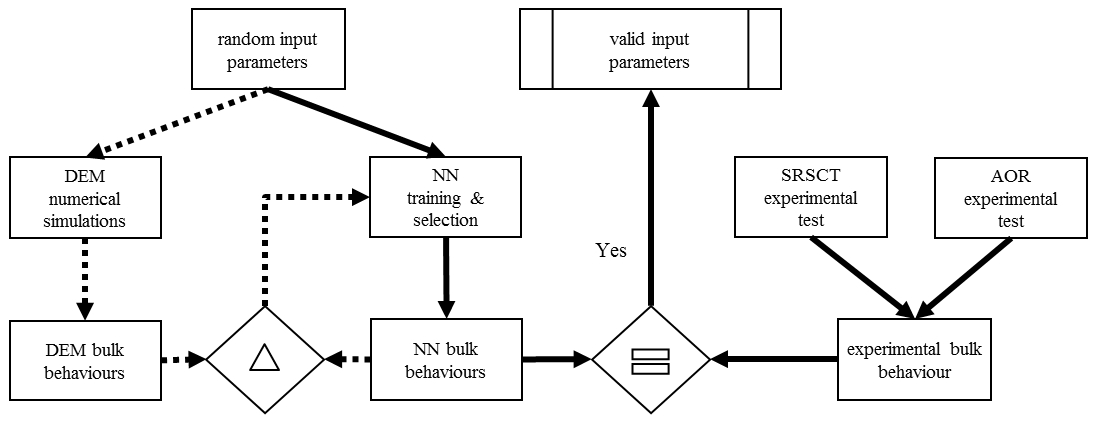
\includegraphics[width=.80\textwidth]{19methodology} 
\caption[Method]{\small{Method. 
In the training phase (dashed lines)
$DEM$ simulations are performed
with random initial input parameters.
The behaviours obtained are used to train the
Artificial Neural Networks ($ANNs$) in a loop that continues until the
difference between the outputs of each $ANN$ and its simulations is below the
limit ($\Delta$) (see Section \ref{subsec:ann}).
In the parameters identification phase (solid
lines) we identify valid input parameters by comparing (\textbf{=}) $ANNs$ and
experimental behaviours.
Further explanations can be found in Section \ref{sec:methodology}.
}}
\label{fig:19methodology} 
\end{figure}
%************************************************
\subsection{Discrete element method}
\label{subsec:dem}

We decided to utilize a single
contact law for all the simulations performed, for details see
Benvenuti et al. \cite{RefWorks:180}.
The $DEM$ parameters for the Young's modulus ($E$) and the Poisson's coefficient
($\nu$) were taken from the literature, see \cite{RefWorks:175} 
and \cite{RefWorks:176}; however we reduced the former to increase the time step
($\Delta t$), following the recommendations of Ai et al. \cite{RefWorks:131}.
The time step was between $1.29 \%$ and $1.53 \%$ of the Rayleigh time, which
also depends on the particle density ($\rho_p$).
Furthermore, we locked the size distribution, which was obtained by experimental
sieving, see Table \ref{tab:09DEMFixedinputvalues}.
In the contact law we used, 
the tangential component of the contact force between two generic particles
($F_t$) is truncated to fulfil:
%************************************************
\begin{equation}
F_{t} \leq \mu_s F_{n},
 \label{eq:force_t}
\end{equation}
%************************************************
where $F_n$ is the normal component and $\mu_s$ is the coefficient of sliding
friction, one of the particle-based $DEM$ parameter we investigated, 
another being the coefficient of rolling friction ($\mu_r$). 
For coarse non-spherical particles, this is a critical parameter and describes
inter-particle friction in medium to dense granular flow simulations. It is proportional to the 
torque counteracting the rotation of the particle. The $\mu_r$ parameter enters the 
equations according to the elasto-rolling resistance model presented by Wensrich and 
Katterfeld \cite{RefWorks:87} and Ai et al. \cite{RefWorks:131} 
based on the work of Jiang et al. \cite{RefWorks:143}. 
The model is called $EPSD2$ in $LIGGGHTS$ and is appropriate for both one-way and cyclical rolling cases.
The maximum magnitude of rolling resistance torque is (Eq. \ref{eq:trmax}):
%************************************************
\begin{equation}
T_{r~max} = \mu_r R_r |\tilde{F_n}| ~,
 \label{eq:trmax}
\end{equation}
%************************************************
where $R_r$ is the equivalent radius and $F_n$ the normal force.
The last two particle-based $DEM$ parameters we investigated were $\rho_p$
and the coefficient of restitution ($COR$) as defined by Ai. et al. \cite{RefWorks:131}.
These coefficients, $COR$, $\mu_s$, $\mu_r$,
$\rho_p$ and $dCylDp$ (the cylinder dimension, proportional to the mean
particle diameter), as indicated in Table \ref{tab:10DEMVariableinputvalues}, 
were constant in each simulation, but their combination differed between
simulations.
Further, $dCylDp$ was used to evaluate the wall effect, but only $~10\%$ of the
simulations had a $dCylDp$ larger than $20$ (additional information can be found
in Benvenuti et al. \cite{RefWorks:180}).
The normal stress $\sigma_n$ and its
percentage during the incipient flow condition $\tau_{\%}$
varied to replicate twelve shear-cell load conditions. 
The complete description of the shear-cell 
and the $AoR$ simulations
can be found in Benvenuti et al. \cite{RefWorks:180}.
A Matlab script allowed us to extract from the simulation output the numerical
values representative of bulk behaviour (hereafter called $bulk ~ values$)
for each DEM simulation parameter combination, which consists of
bulk density ($\rho_b$),
coefficient of internal friction in the pre-shear phase ($\mu_{psh}$),
coefficient of internal friction in the shear phase ($\mu_{sh}$),
and angle of repose ($AoR$).
The first bulk value ($\rho_b$) was provided directly. 
For correctly performed simulations, see Benvenuti et al. \cite{RefWorks:180}, we
observed a stress path as in Fig. \ref{fig:21simexample}.
First, the $\sigma_n$ was kept constant while the coefficient of internal
friction ($\mu_{ie}$) initially increased and then reached a plateau.
The second bulk value ($\mu_{psh}$) was calculated as the average of the
$\mu_{ie}$ in this plateau.
The $\sigma_n$ was then automatically reduced, in our example to $80 \%$ of
its initial value.
Subsequently, a second plateau developed.
We obtained the third
value ($\mu_{sh}$) as the average of $\mu_{ie}$ in this second plateau.
The stress path accords with the experimental one, especially the plateaux.\\
In the $AoR$ tests the average of the repose angles provided us with the fourth
bulk value, allowing us to define the numerical bulk behaviour.
%************************************************
\begin{figure}[htp] \centering
    \begin{subfigure}[b]{0.45\textwidth}
        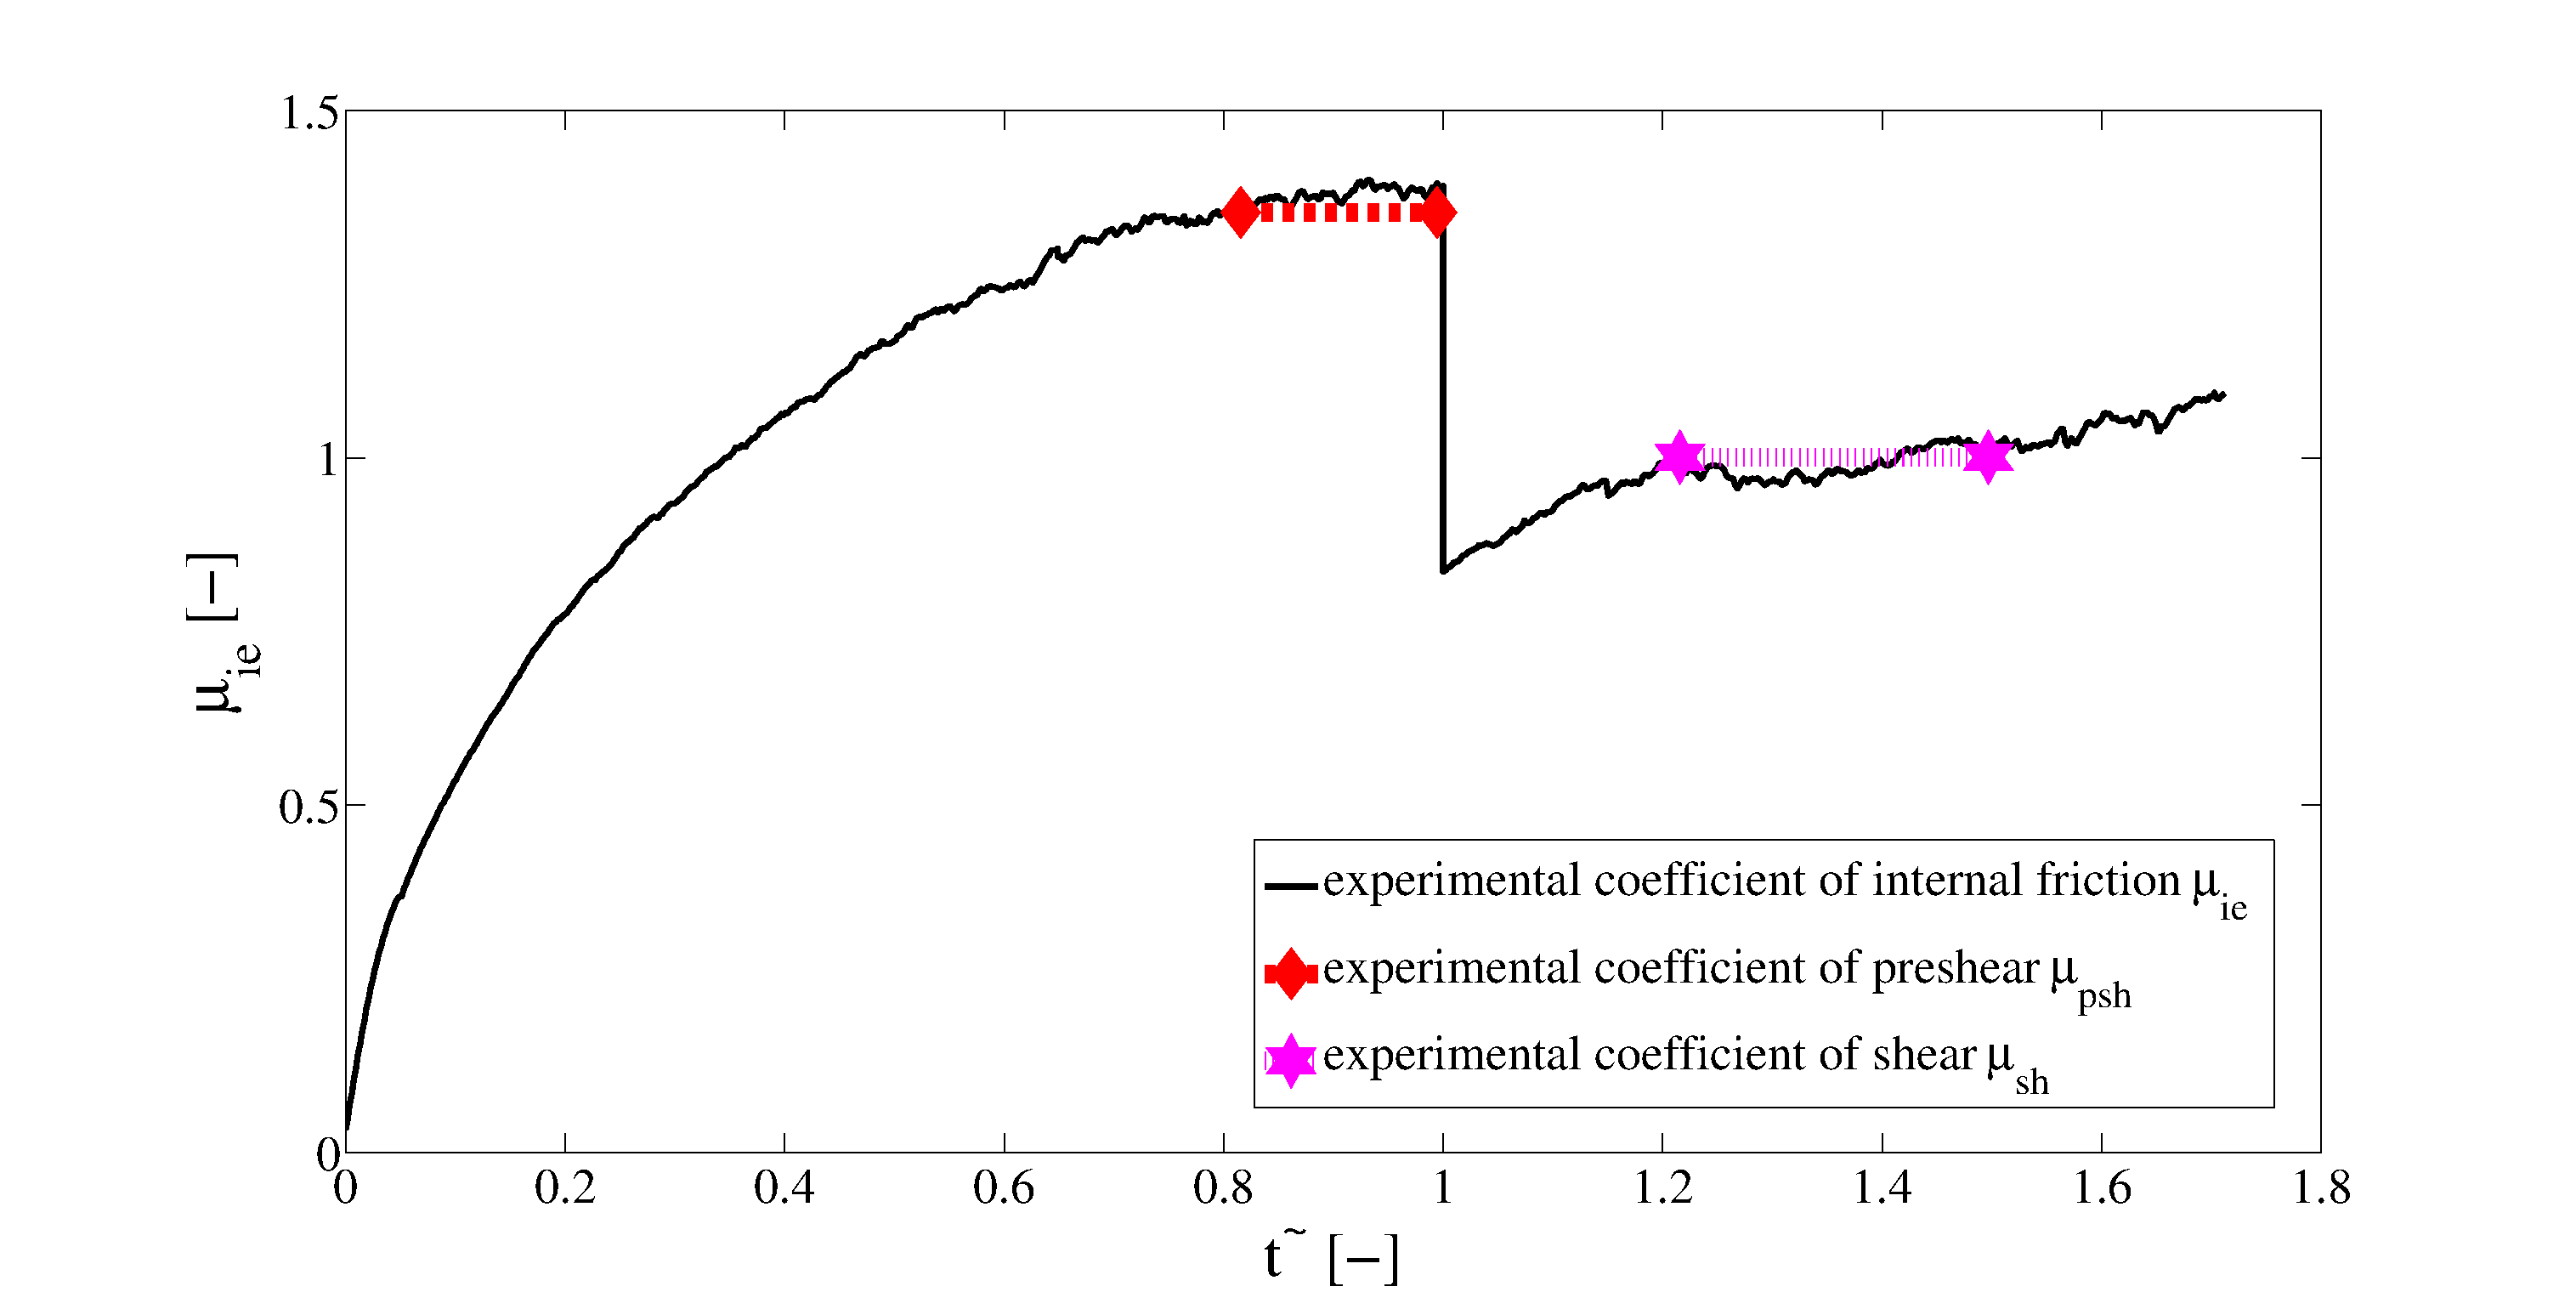
\includegraphics[width=\textwidth]{20experimental}
        \caption{Experimental shear-cell tester stress path - $\sigma_n =
         10000
        ~Pa$}
        \label{fig:20experimental} 
    \end{subfigure}
        \begin{subfigure}[b]{0.45\textwidth}
        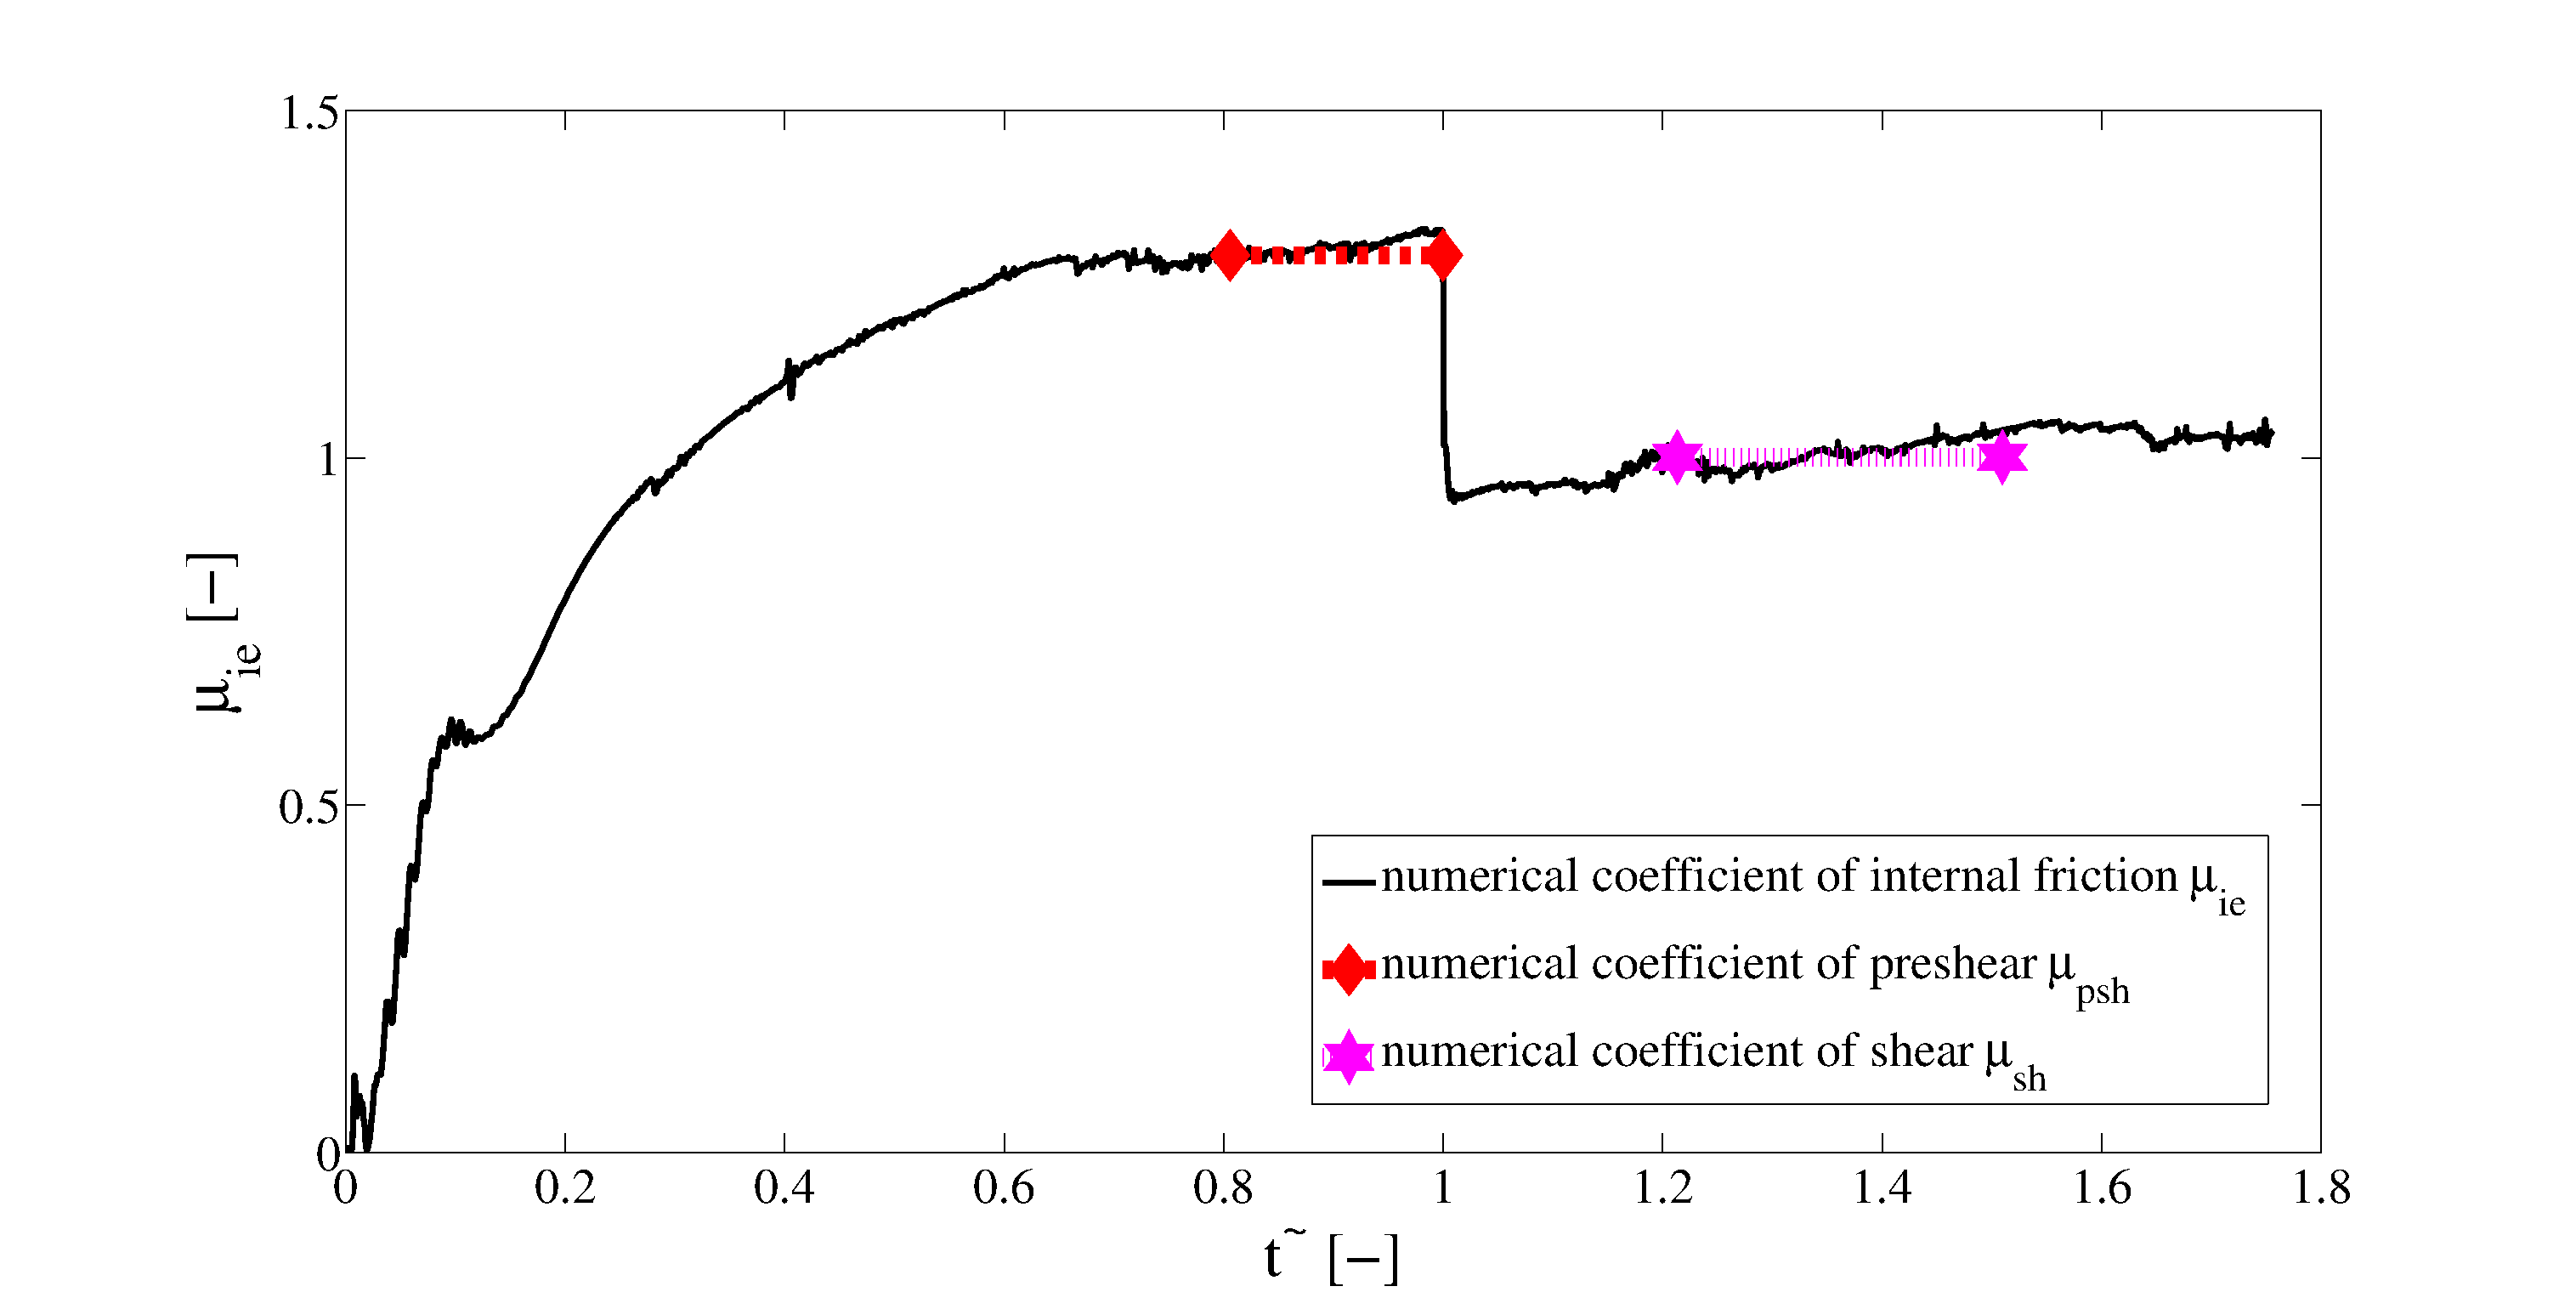
\includegraphics[width=\textwidth]{21simexample}
        \caption{Numerical shear-cell tester stress path - $\sigma_n = 10000
        ~Pa$}
        \label{fig:21simexample} 
    \end{subfigure}
    \caption[Stress path]{\small{Experimental and numerical samples of the
    stress path for the Schulze ring shear cell tester.
	Time was normalized: $\tilde{t} = t/t_{change}$, where $t_{change}$ is the
	point in time at which the normal stress ($\sigma_n$) was modified during the
	tests.
	Until $\tilde{t}=1$, the $\sigma_n$ was kept constant at 10,000 Pa. 
	In Fig. \ref{fig:20experimental}, 
 	a plateau was reached at $\tilde{t}~=0.91$.
	The coefficient of pre-shear ($\mu_{psh}$) was calculated as the average of the
	coefficient of internal friction ($\mu_{ie}$) in this first plateau.
	At $\tilde{t}=1$, the $\sigma_n$ was reduced to $80 \%$ of its initial
	value, and soon after
	a second plateau developed.
	We obtained the coefficient of
	shear ($ \mu_{sh}$) as the average of $\mu_{ie}$ in this second plateau.
	The stress paths agree well, especially the plateaux.
	They were clearly relevant because
	the values representative of the bulk behaviours 
	were collected there.}}
    \label{fig:40experimentalsimulation}
\end{figure}
%************************************************
\begin{table}[h]
\centering
\scalebox{0.8}{
\begin{tabular}{ccccc}
\hline
    Mean & Std.dev.  & Young's & Poisson's & $\Delta t$\\
    $R$ & $R$ & modulus & ratio & \\
    (mm)  & (mm)  & (MPa) & (-) & (s)\\
    \hline
    $0.732$ & $0.41$ & $10$    & $0.40$ & $10^{-6}$\\
\hline
\end{tabular}}
\caption{\small{DEM fixed input values}}
\label{tab:09DEMFixedinputvalues}
\end{table}
%************************************************
\begin{table}[h]
\centering
\scalebox{0.8}{
\begin{tabular}{ccccc}
\hline
    $\mu_s$ & $\mu_r$ & $COR$ & $\rho_p$ & $dCylDp$ \\
    	(-)  & (-)   & (-)   & (kg/m3) & (-) \\
    \hline
    0.4 / 0.6 / 0.8 & 0.4 / 0.6 / 0.8 & 0.5 / 0.7 / 0.9 & 2500 / 3000 / 3500 & 20 / 36 / 38 / 40 \\

\hline
\end{tabular}}
\caption[DEM variable input values]{\small{DEM variable input values for
training the Artificial Neural Networks}}
\label{tab:10DEMVariableinputvalues}
\end{table}
%************************************************
\begin{table}[h]
\centering
\scalebox{0.8}{
\begin{tabular}{lcccc}
\hline
 &  $\mu_s$ & $\mu_r$ & $COR$ & $\rho_p$  \\
   &	(-)  & (-)   & (-)   & (kg/m3) \\
          \hline
    range & $[0.1 \ldots 1.0]$ & $[0.1 \ldots 1.0]$ & $[0.5 \ldots 0.9]$ &
    $[2000 \ldots 3500]$     \\
    number of values & 100   & 100   & 25    & 25    \\

\hline
\end{tabular}}
\caption[DEM random input values]{\small{DEM random input values. Within each
range the indicated number of random values was chosen according to a standard uniform
distribution.}}
\label{tab:12DEMRandominputvalues}
\end{table}
%************************************************

\subsection{Artificial Neural Networks}
\label{subsec:ann}
We first defined the typology of Artificial Neural Networks ($ANNs$) we used and
the input we fed them, see Benvenuti et al. \cite{RefWorks:180}.
Our $ANNs$ have three different layers: the input layer has a number of neurons
equal to the number of different inputs of the network.
%, see Fig. \ref{fig:18nnscheme}.
The hidden (or central) layer's number of neurons was to be investigated. 
The output layer contains one neuron for the output.
The transfer functions between the first two layers are the tangential sigmoid, 
and those between the hidden and central layers are linear.\\
Thus, we were able to use the $DEM$ parameter combinations and their
corresponding bulk values to train the $ANNs$.
Note that 15\% of the simulations ($test ~ simulations$) were
randomly picked and excluded from the training processes.
We started with all the $DEM$ parameter combinations and their corresponding
numerical $\mu_{psh}$ to create 36 $ANNs$ that differed in their numbers of
neurons in the hidden layer (between five to forty neurons).
We then determined the coefficient of determination ($R^2$) between the
$bulk-macro$ behaviours in the output of the $ANN$ and the 15\% $test ~ simulations$, 
which were not correlated with the remaining 85\% used for the training. 
Thus, we could select for $\mu_{psh}$ the $ANN$ with the maximum $R^2$, 
again as suggested by Vaferi et al. \cite{RefWorks:150}, and we noted its number
of neurons.
We repeated the same $ANN$ creation steps for $\mu_{sh}$, $\rho_b$
and $AoR$, obtaining one trained $ANN$ for each bulk value. \\
Since $\mu_{psh}$, $\mu_{sh}$ and $\rho_b$ belonged to the shear-cell
simulations, their $ANNs$ were handled together: we had one cluster with three 
$ANNs$ for the shear cell and one with only one $ANN$ for the $AoR$.
We could then proceed in identifying valid input parameters.
Oberkampf et al. \cite{RefWorks:160} suggested using a Design of Experiments
($DoE$) method to determine the parameter combinations to be simulated.
They stated that this approach allows optimization of computation time
with an acceptable loss of precision.
The speed of the trained $ANNs$ enabled us to follow a different approach to
maximizing the precision of the characterization.
We created random values
in the range and numbers defined in Table \ref{tab:12DEMRandominputvalues}
according to a standard uniform distribution.
The total number of combinations of these random values was 6,250,000.
These combinations were then fed to and processed by the selected
$ANNs$, and thus three bulk values for the shear
cell and one for the $AoR$ were obtained.
%************************************************
% \begin{figure}[!htb] 
% \centering 
% 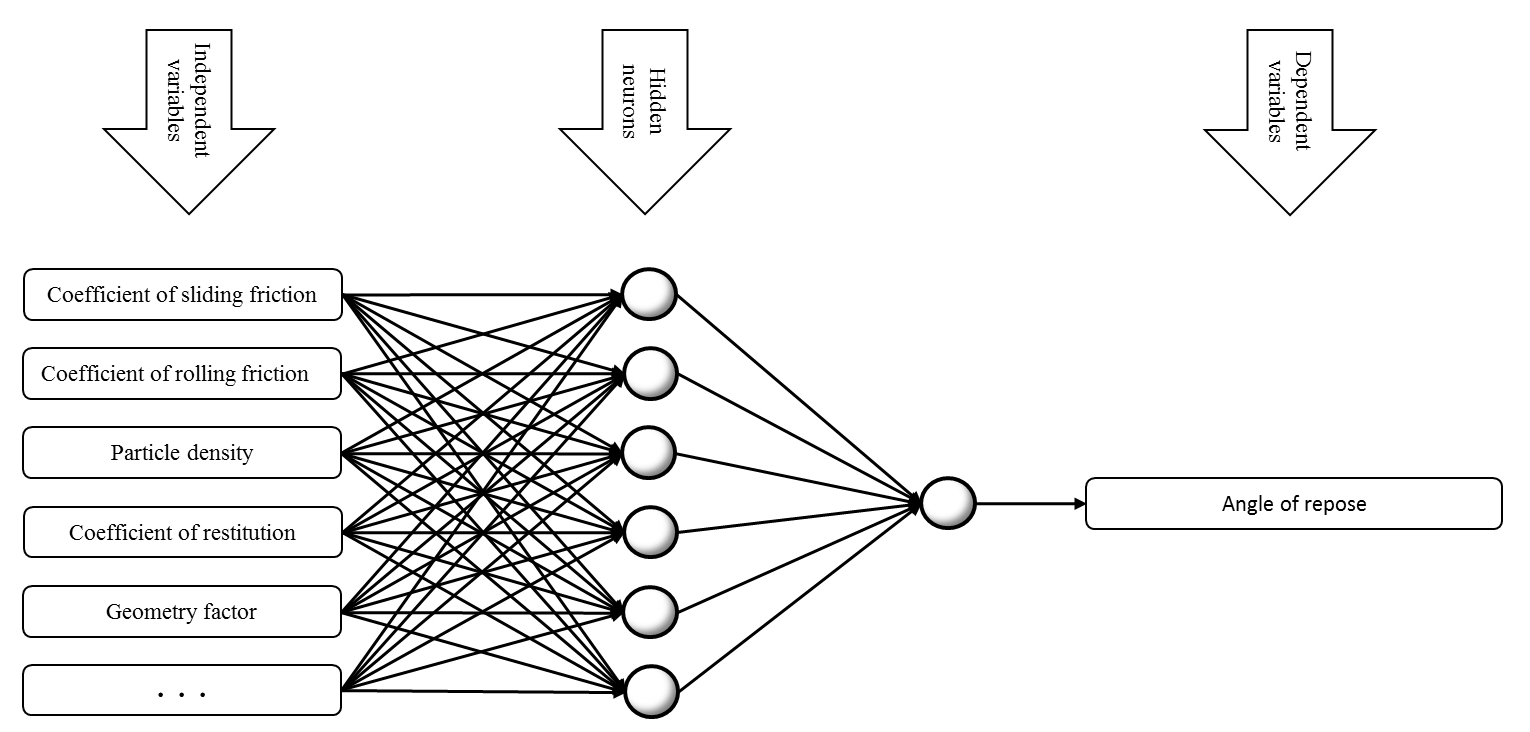
\includegraphics[width=.8\textwidth]{18nnscheme} 
% \caption[ANN Scheme]{Artificial Neural Network ($ANN$) Scheme
% of how the Multilayer Perceptron $ANN$ ($MLPNN$) derives one
% bulk-behaviour-dependent variable from the mutually independent simulation variables.}
% \label{fig:18nnscheme} 
% \end{figure}
%************************************************

\subsection{Macroscopic Experiments and Parameter Identification}
\label{subsec:macroscopicexperimentsparameteridentification}
The experimental characterization was performed as described in
Benvenuti et al. \cite{RefWorks:180}. 
We obtained for each of the twelve load conditions of the $SSC$ three bulk
values ($\mu_{psh}$, $\mu_{sh}$ and $\rho_b$).
The fourth bulk value was the result of two angle of repose ($AoR$) tests that
recreated the repose angle observed in a pile of the
real material. 

Subsequently, we compared the $ANN$ and experimental bulk behaviours for the
twelve shear-cell load conditions.
If in a DEM-parameter combination all the three bulk values differed by less 
than 5\% from those of the corresponding experiments, i.e.:
%************************************************
\begin{equation}
 \begin{cases}
\text{if } & \lvert{1-\frac{\mu_{psh,num}}{\mu_{psh,exp}}}\rvert < 5\%  ,\\
\text{and if } & \lvert{1-\frac{\mu_{sh,num}}{\mu_{sh,exp}}}\rvert < 5\% , \\ 
\text{and if } & \lvert{1-\frac{\rho_{p,num}}{\rho_{p,exp}}}\rvert < 5\% ,\\ 
\end{cases}
 \label{eq:check2}
\end{equation}
%************************************************
the combination was marked. The marked combinations were processed by the
$AoR$ $ANN$, and then compared with the experiment.
Were considered valid those that differed by less than $5\%$ also in this
comparison (Eq. \ref{eq:checkaor}):
%************************************************
\begin{equation}
\text{if} ~~~~~~ \lvert{1-\frac{AoR_{num}}{AoR_{exp}}}\rvert < 5\% .
\label{eq:checkaor}
\end{equation}
%************************************************
Further, to prove the validity of the system, we tested the marked combinations
by modifying the experimental bulk values of the shear cell. 
We artificially decreased or increased the shear force, and thus $\mu_{psh}$ and
$\mu_{sh}$, by a product coefficient ($P$), e.g. 
%Eq. \ref{eq:pcoeff}:
$\mu_{psh, new} = \mu_{psh, old} \cdot P$.
%************************************************
% \begin{equation}
% \label{eq:pcoeff}
% \mu_{psh, new} = \mu_{psh, old} \cdot P .
% \end{equation}
%************************************************

\section{Results and discussion}
\label{sec:results}
%************************************************

\subsection{DEM Simulations}
\label{subsec:simulations}

For sinter fine, 546 shear cell and 81 static $AoR$ simulations were run with
the parameter combinations described in Table
\ref{tab:10DEMVariableinputvalues}.
The computational time amounted to 1 hour with 32 AMD cores for a benchmark
shear-cell simulation and to 9 hours for a benchmark $AoR$ simulation, both with
50,000 particles.
Simulations with larger $dCylDp$ required more time (e.g., about 12 hours for
the shear cell with 400,000 particles ). \\


\subsection{ANN model development}
\label{subsec:annmodeldev}

First, we determined the regression of the bulk behaviour parameters, for
instance the $\mu_{psh}$. 
% see Fig. \ref{fig:22regression}, where the
% corresponding plot for the $ANN$ with the maximum $R^2$ is shown. Each circle represents one of the 546
% simulations.
The plot shows a consistent agreement between the 
$DEM$ and the $ANN$ values and an almost linear regression ($R^2
= 0.94$).
% The linear relationship between the
% training values can be seen in Table \ref{tab:06inputRelationshipTable}.
% The clearest connections were between $\mu_s$ and $\mu_{psh}$, and
% $\rho_p$ and $\rho_b$.
% In contrast, for $\mu_{sh}$ and $AoR$, the $\mu_r$ balanced the influence of the 
% $\mu_s$. \\
We then investigated how the $R^2$ changed with the number of neurons
for the $\mu_{psh}$.
In this case, we achieved a $R^2 = 0.96$ for an $ANN$ with fifteen neurons. 
Increasing the number of neurons did not improve the $R^2$; it even started to
oscillate with higher numbers of neurons.
We subsequently obtained the optimal number of neurons for all $ANNs$.
Further, we processed the random combinations (Table
\ref{tab:10DEMVariableinputvalues}) with the $ANN$.
The $ANN$ evaluation was significantly faster than the $DEM$ simulations. The
individuation of the numerical bulk behaviours for all the $DEM$ combinations
did not take more than a few seconds on a single core.
%************************************************
% \begin{figure}[!h] 
% \centering 
% 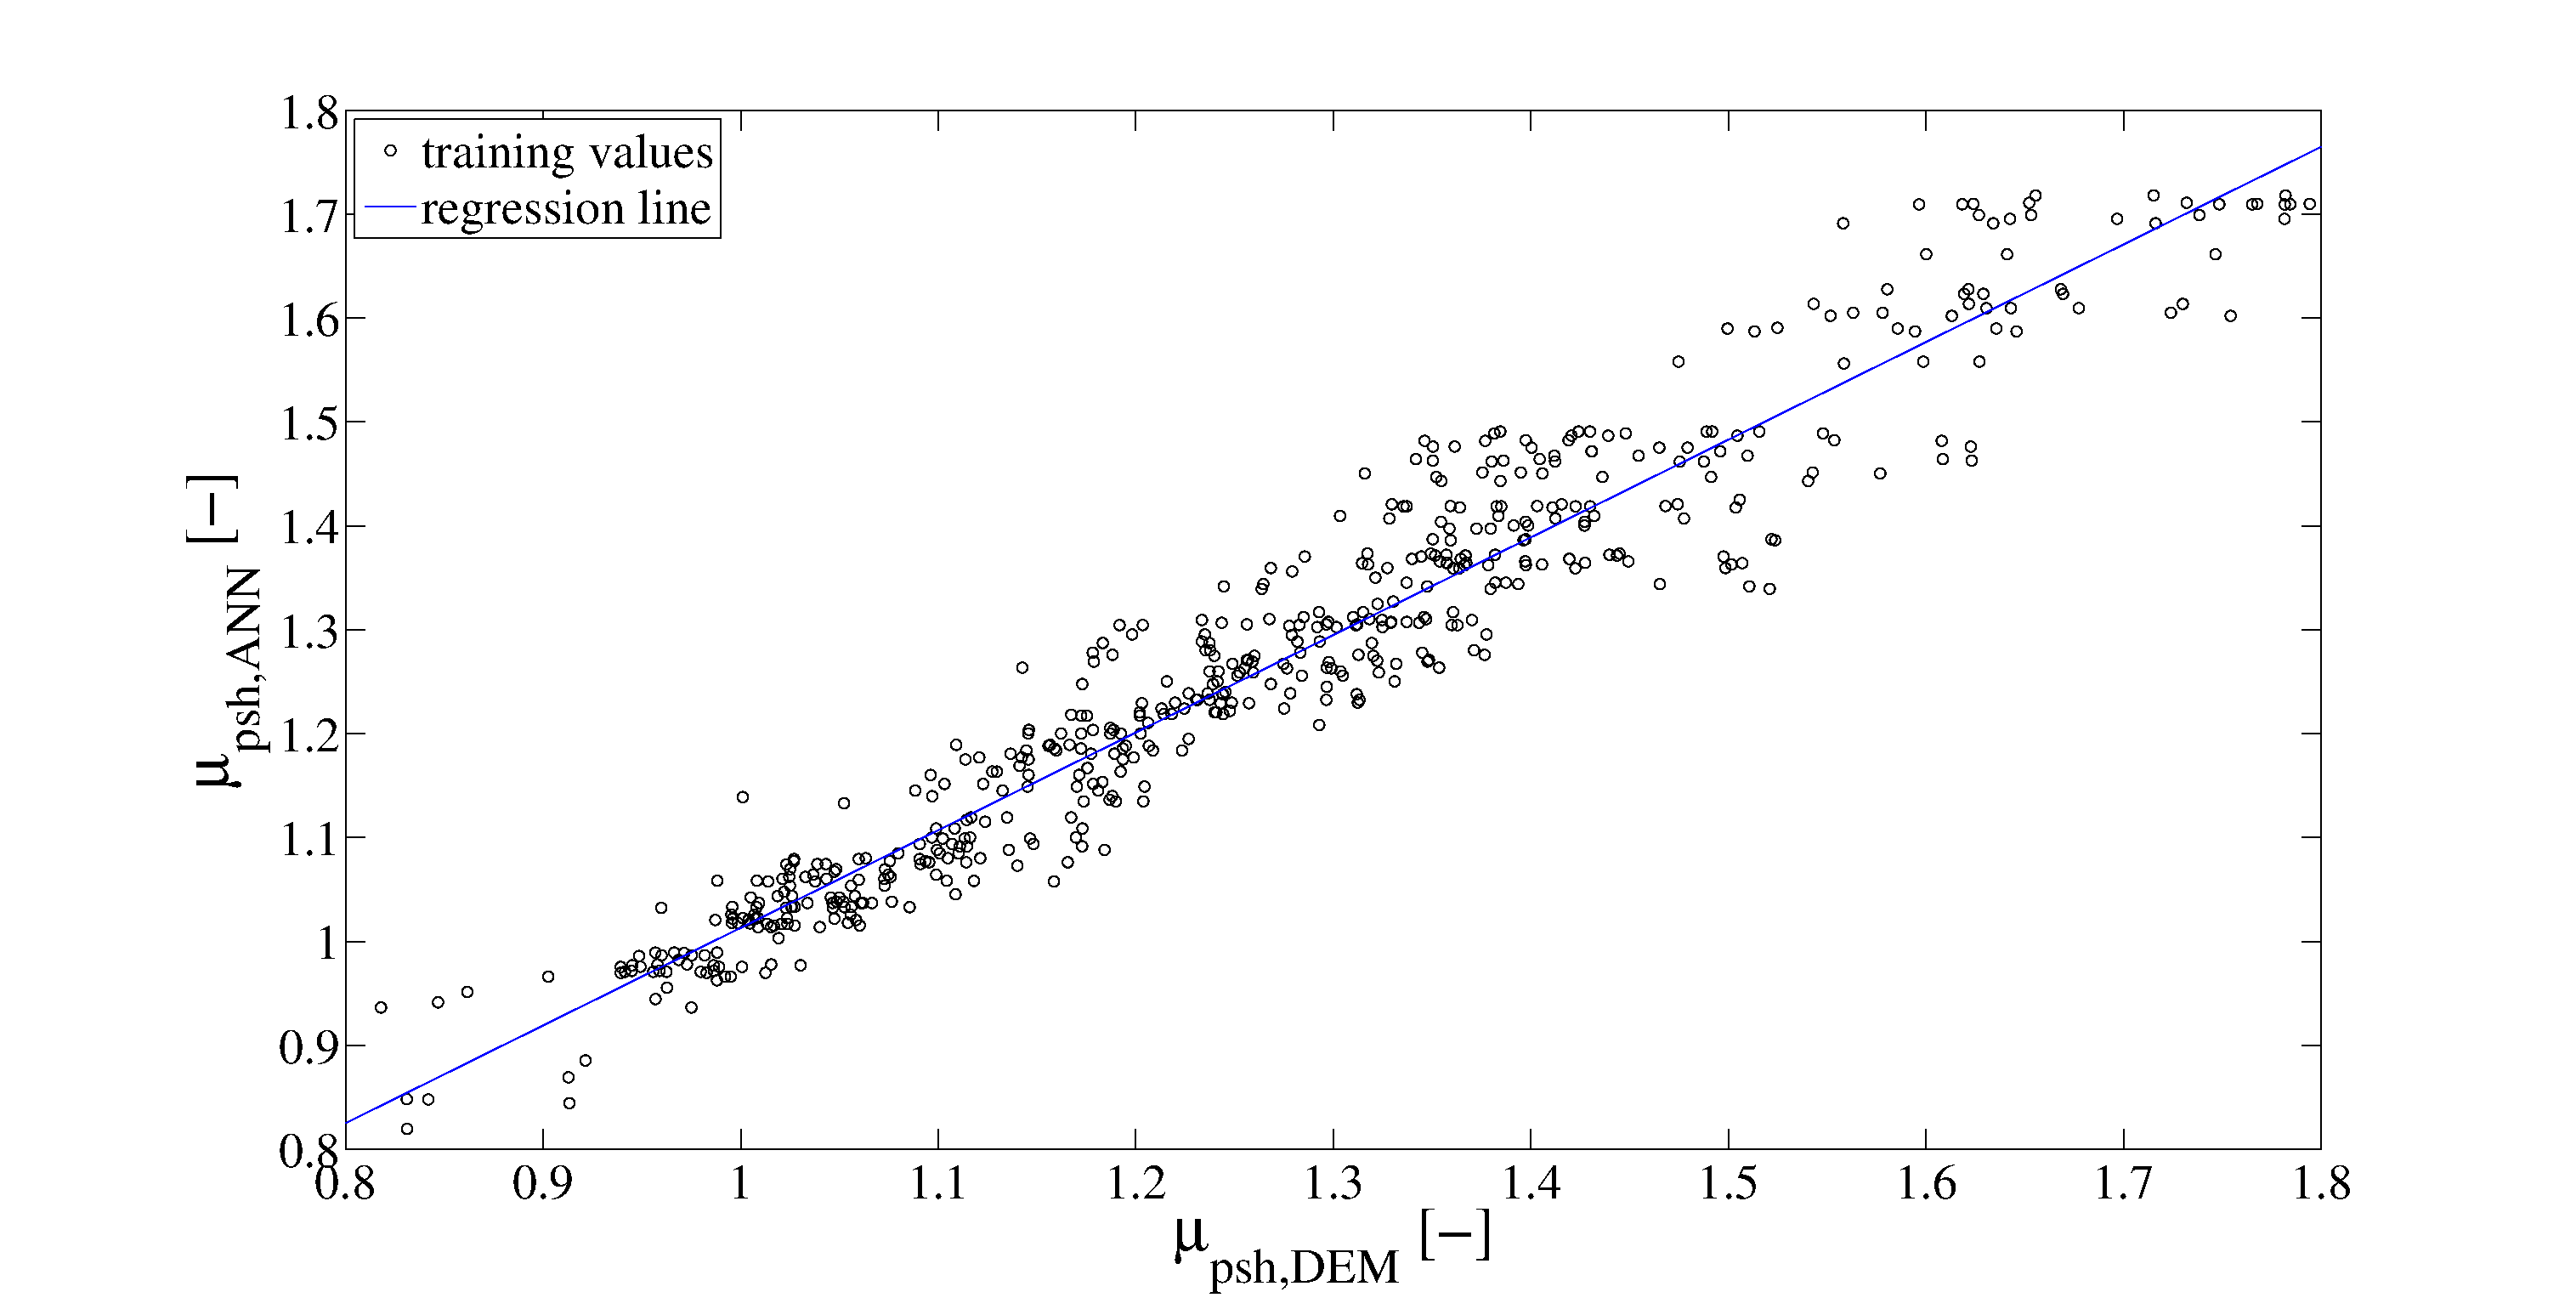
\includegraphics[width=.96\textwidth]{22regression}
% %[width=.96\textwidth]
% \caption[Comparison between prediction of the trained ANN and full DEM
% simulation]{Comparison between prediction of the trained Artificial Neural
% Network ($ANN$) and 546 full DEM simulations of the coefficient of pre-shear
% ($\mu_{psh}$). In this case the regression line is nearly linear (0.94), and
% demonstrates the accurate predictive power of the $ANN$.}
% \label{fig:22regression} 
% \end{figure}
%************************************************
% \begin{table}[h]
% \centering
% \scalebox{1.0}{
% \begin{tabular}{lcccccccc}
% \hline
%          & $\mu_s$ & $\mu_r$ & $COR$ & $\rho_p$ & $\mu_{sh}$ &
%         $\mu_{psh}$ & $\rho_{b}$ & $AoR$ \\
%           \hline
%     $\mu_s$ & 100.00 & 0.55  & 0.04  & 0.00  & 3.84  & 87.26 & 8.39  & 49.48 \\
%     $\mu_r$ & 0.55  & 100.00 & 0.15  & 0.00  & 58.92 & 33.70 & 3.10  & 60.20 \\
%     $COR$ & 0.04  & 0.15  & 100.00 & 0.00  & 15.52 & 0.57  & 1.71  & 21.35 \\
%     $\rho_p$ & 0.00  & 0.00  & 0.00  & 100.00 & 4.98  & 5.71  & 99.00 & 0.00 \\
%     $\mu_{sh}$ & 3.84  & 58.92 & 15.52 & 4.98  & 100.00 & 26.03 & 9.52  & 0.00 \\
%     $\mu_{psh}$ & \textbf{87.26} & 33.70 & 0.57  & 5.71  & 26.03 & 100.00 & 4.33 
%     & 0.00
%     \\
%     $\rho_{b}$ & 8.39  & 3.10  & 1.71  & \textbf{99.00} & 9.52  & 4.33  & 100.00
%     & 0.00 \\
%     $AoR$ \hspace{5ex} & 49.48 & \textbf{60.20} & 21.35  & 0.00  & 0.00  & 0.00 
%     & 0.00  & 100.00 \\
%     
% \hline
% \end{tabular}}
% \caption[Values of linear relationship between considered variables]{Values of
% linear relationship between variables considered multiplied by 100. Sliding
% friction ($\mu_s$), rolling friction ($\mu_r$) and particle density ($\rho_p$)
% had the greatest influence on, respectively, the coefficient of pre-shear
% ($\mu_{psh}$), the angle of repose  ($AoR$) and the bulk density ($\rho_b$). Notably, $\rho_p$
% was not used as a training parameter for $AoR$ bulk behaviour.}
% \label{tab:06inputRelationshipTable}
% \end{table}
%************************************************


\subsection{Experiments and Parameter Identification}
\label{subsec:experimentsparameteridentification}

Experimental values identifying the bulk behavior, $\mu_{psh}$, $\mu_{sh}$ and $\rho_{b}$, 
of sinter fine were acquired through $SSC$ tests. 
Table \ref{tab:05sinterTableExperimental} presents
these values for three load conditions: clearly the $\mu_{psh}$ decreases, and 
the $\mu_{sh}$ oscillates.
The $\rho_b$ has a clear average of 1,760 kg/m3 with a 42 
kg/m3 deviation.
The stress path for the second load condition in Table
\ref{tab:05sinterTableExperimental} is shown in Fig.
\ref{fig:20experimental}.
Two $AoR$ tests were performed that gave an average angle of
38.85$^\circ$.
We obtained the radius ($R$) mean and standard
deviations, as shown in Table
\ref{tab:09DEMFixedinputvalues}, from sieving experiments.
The comparison between numerical and experimental behaviours led to a first
series of marked combinations ($MC1$) for one load condition of
the shear cell ($\sigma_n=10,070$ Pa, P=1.0), as plotted in Fig.
\ref{fig:24radarpirker1schulze10070}, where 
the minimum and maximum values are shown, together with the mean. 
Note that the confidence interval is large, 
especially for the $COR$, which highlights its insignificant influence on the
characterization.
Both the $\rho_p$  and the $\mu_s$, however, show a narrow confidence interval, 
which demonstrates their influence and the ability of this procedure to find
valid $DEM$ parameters.
These results agree with our examination of the ratio of the standard deviation
to the range, see Table \ref{tab:13DEMvalidvalues}.
Further, we observed that various $DEM$ parameter
combinations could reproduce the experimental behaviour, and thus evaluated
their mutual dependencies.
This is shown more clearly in a density plot (see Fig. 
\ref{fig:25cloudpirker1schulze10070} for $MC1$) 
of the particles' coefficient of restitution (COR) in relation to
the coefficients of sliding friction ($\mu_s$) and rolling friction ($\mu_r$). 
Multiple
combinations (250,407 or 4\% of the total) of $\mu_s$ and $\mu_r$ reproduced
the experimental behaviour with varying $COR$.
This underlines once more their correlation, as already stated by Wensrich and 
Katterfeld \cite{RefWorks:87}.
To further demonstrate the validity of the procedure, we modified the product
coefficient. 
First, we set it to $P=0.8$, and we obtained another
series of marked combinations ($MC2$).
It can be seen in the parameter space plot in Fig.
\ref{fig:26radarpirker08schulze10070} that the confidence range is narrower
than for $P=1.0$, while in the density plot in Fig. 
\ref{fig:27cloudpirker08schulze10070} the area
appears larger, although slightly less densely populated. Finally, for $P=1.2$
and its marked combinations ($MC3$) the parameter space plot in Fig.
\ref{fig:28radarpirker12schulze10070} shows a largely different confidence
range, while the density plot in Fig. \ref{fig:30cloudpirker12schulze10070} 
shows a smaller area. As expected, the procedure was highly sensitive to
variations in the experimental data.
Our approach could therefore be used
for a wide range of bulk materials.\\
We then processed the random combinations with the $AoR$ $ANN$. In Fig.
\ref{fig:31radarpirker1aor} the parameter space plot for the same criteria as
before can be seen.
In accordance with theory (Wensrich and Katterfeld \cite{RefWorks:87}), in a simulation dominated
by rolling particles, the coefficient of rolling friction has the maximum
influence. \\
Finally, we extracted from the $MC1$ values the $AoR$ $ANN$ behaviour
and compared it with the experimental one.
As can be seen in the parameter space plot in Fig.
\ref{fig:33radarpirker1schulze10070aor}, the confidence interval is very small,
indicating that all the parameters but the $COR$ played an important role, 
and demonstrating the reliability of these parameter
combinations in representing the bulk behaviour.
From the initial 6,250,000 combinations, only 3,884 were valid (0.0621
\%), see Table \ref{tab:13DEMvalidvalues}.
%************************************************
\begin{table}[h]
\centering
\scalebox{0.8}{
\begin{tabular}{cccccc}
\hline
$\sigma_n$ (Pa) & $\tau$ (Pa) & $\mu_{psh}$ (-) & $\tau_{\%}$ (\%) &
$\mu_{sh}$ (-) & $\rho_b$ (kg/m3) \\
\hline
    1068  & 1059  & 0.9916 & 80 & 1.2333 & 1718 \\
    2069  & 1818  & 0.8787 & 80 & 0.9994 & 1759 \\
    10070 & 8232  & 0.8175 & 80 & 1.1712 & 1802 \\

\hline
\end{tabular}}
\caption[Experimental results]{\small{Experimental results. Values for three
load conditions}}
\label{tab:05sinterTableExperimental}
\end{table}
%************************************************
\begin{table}[h]
\centering
\scalebox{0.8}{
\begin{tabular}{llccc}
\hline

          & type  & SSC & AoR   & SSC \& AoR \\
          \hline

    $\mu_s$ & mean  & 0.831 & 0.177 & 0.664 \\
    $(-)$   & std. dev. (SD) & 0.097 & 0.095 & 0.029 \\
          & range ($R$) & 0.9   & 0.9   & 0.9 \\
          & SD / R & 0.108 & 0.106 & 0.032 \\
          \hline
    $\mu_r$ & mean  & 0.692 & 0.830 & 0.916 \\
    $(-)$   & std. dev. (SD) & 0.215 & 0.193 & 0.042 \\
          & range ($R$) & 0.9   & 0.9   & 0.9 \\
          & SD / R & 0.239 & 0.214 & 0.046 \\
          \hline
              COR   & mean  & 0.708 & 0.590 & 0.590 \\
    $(-)$   & std. dev. (SD) & 0.104 & 0.073 & 0.065 \\
          & range ($R$) & 0.4   & 0.4   & 0.4 \\
          & SD / R & 0.259 & 0.183 & 0.161 \\
          \hline
    $\rho_p$ & mean  & 2245.7 & 3192.8 & 2283.9 \\
    $(kg/m3)$ & std. dev. (SD) & 80.5  & 277.4 & 67.1 \\
          & range ($R$) & 1500  & 1500  & 1500 \\
          & SD / R & 0.054 & 0.185 & 0.045 \\
          \hline
    valid & number & 290203 & 816552 & 3884 \\
    combinations & (\%) & 4.64  & 13.06 & 0.06 \\  

\hline
\end{tabular}}
\caption[Valid DEM values]{\small{Valid DEM values. For each parameter we show
the valid parameter statistics in the two tests and in their intersection.
Finally, we show the number of valid parameter combinations over the total
(6250000).}}
\label{tab:13DEMvalidvalues}
\end{table}
%************************************************
\begin{figure}[htp] \centering
        \begin{subfigure}[b]{0.32\textwidth}
        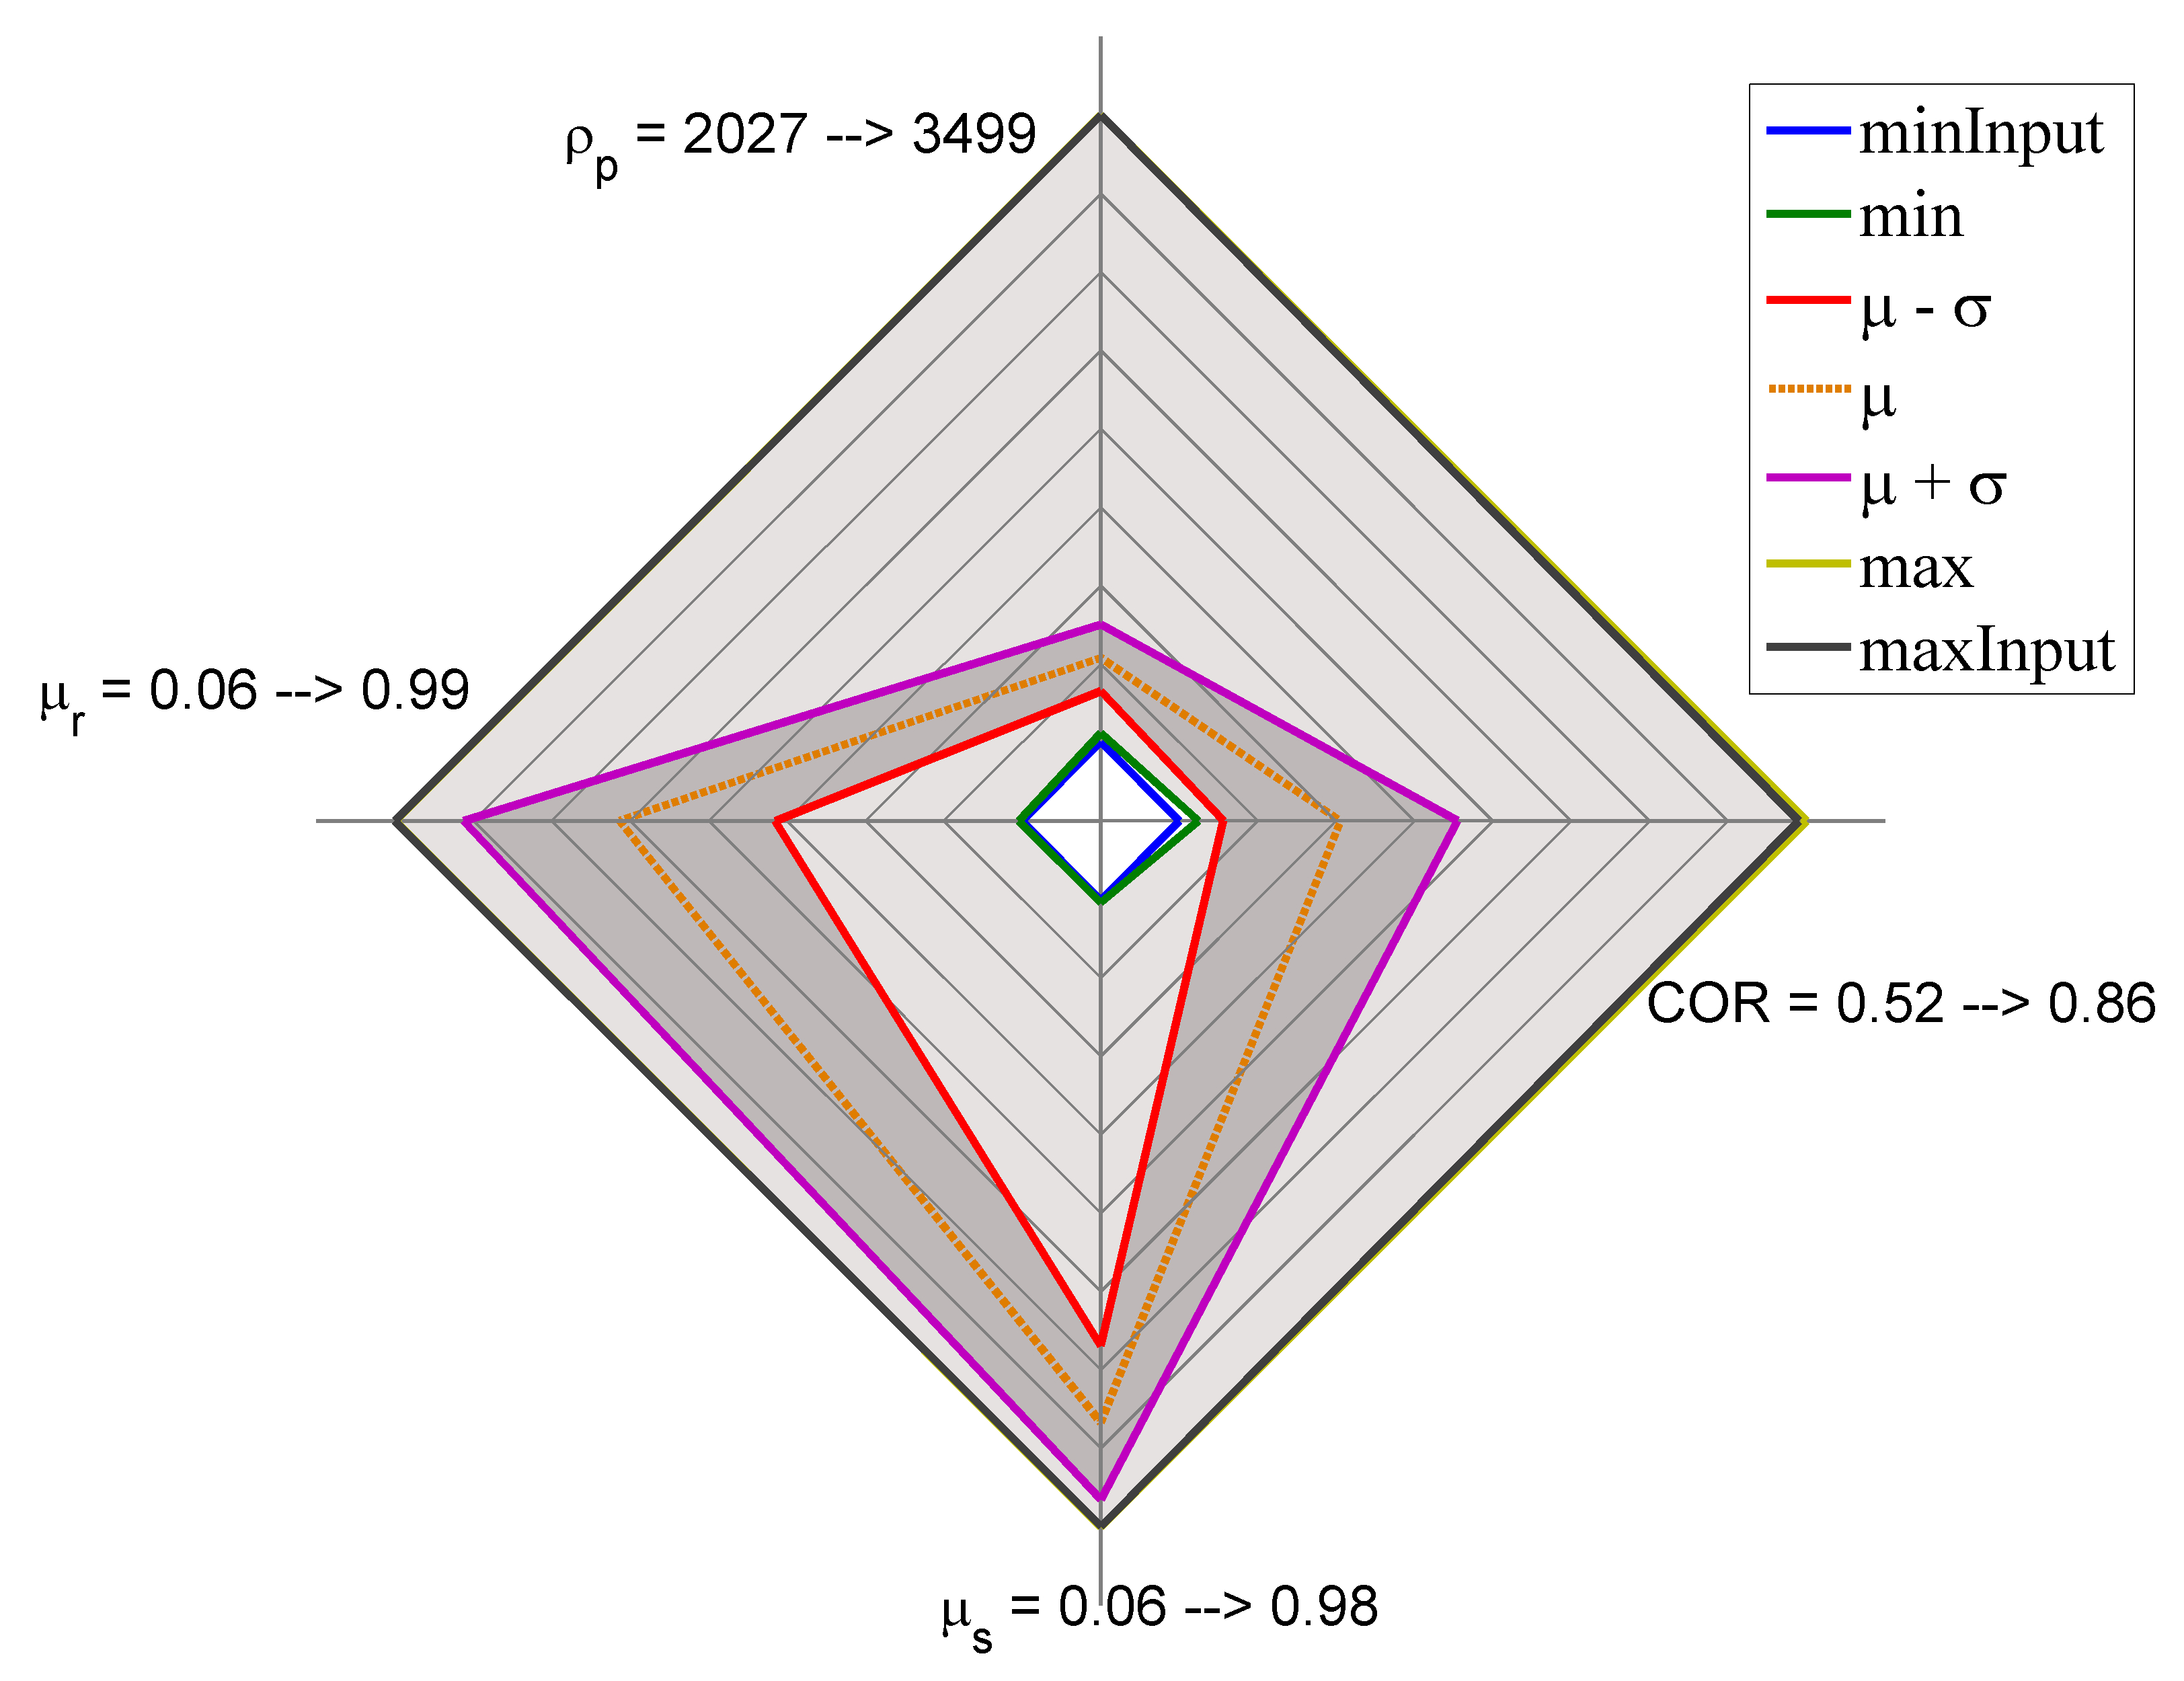
\includegraphics[width=\textwidth]{26radarpirker08schulze10070}
        \caption{Parameter space plot, $SSC$, $\sigma_n=10070$ Pa, P=0.8}
        \label{fig:26radarpirker08schulze10070} 
    \end{subfigure}
     \begin{subfigure}[b]{0.32\textwidth}
        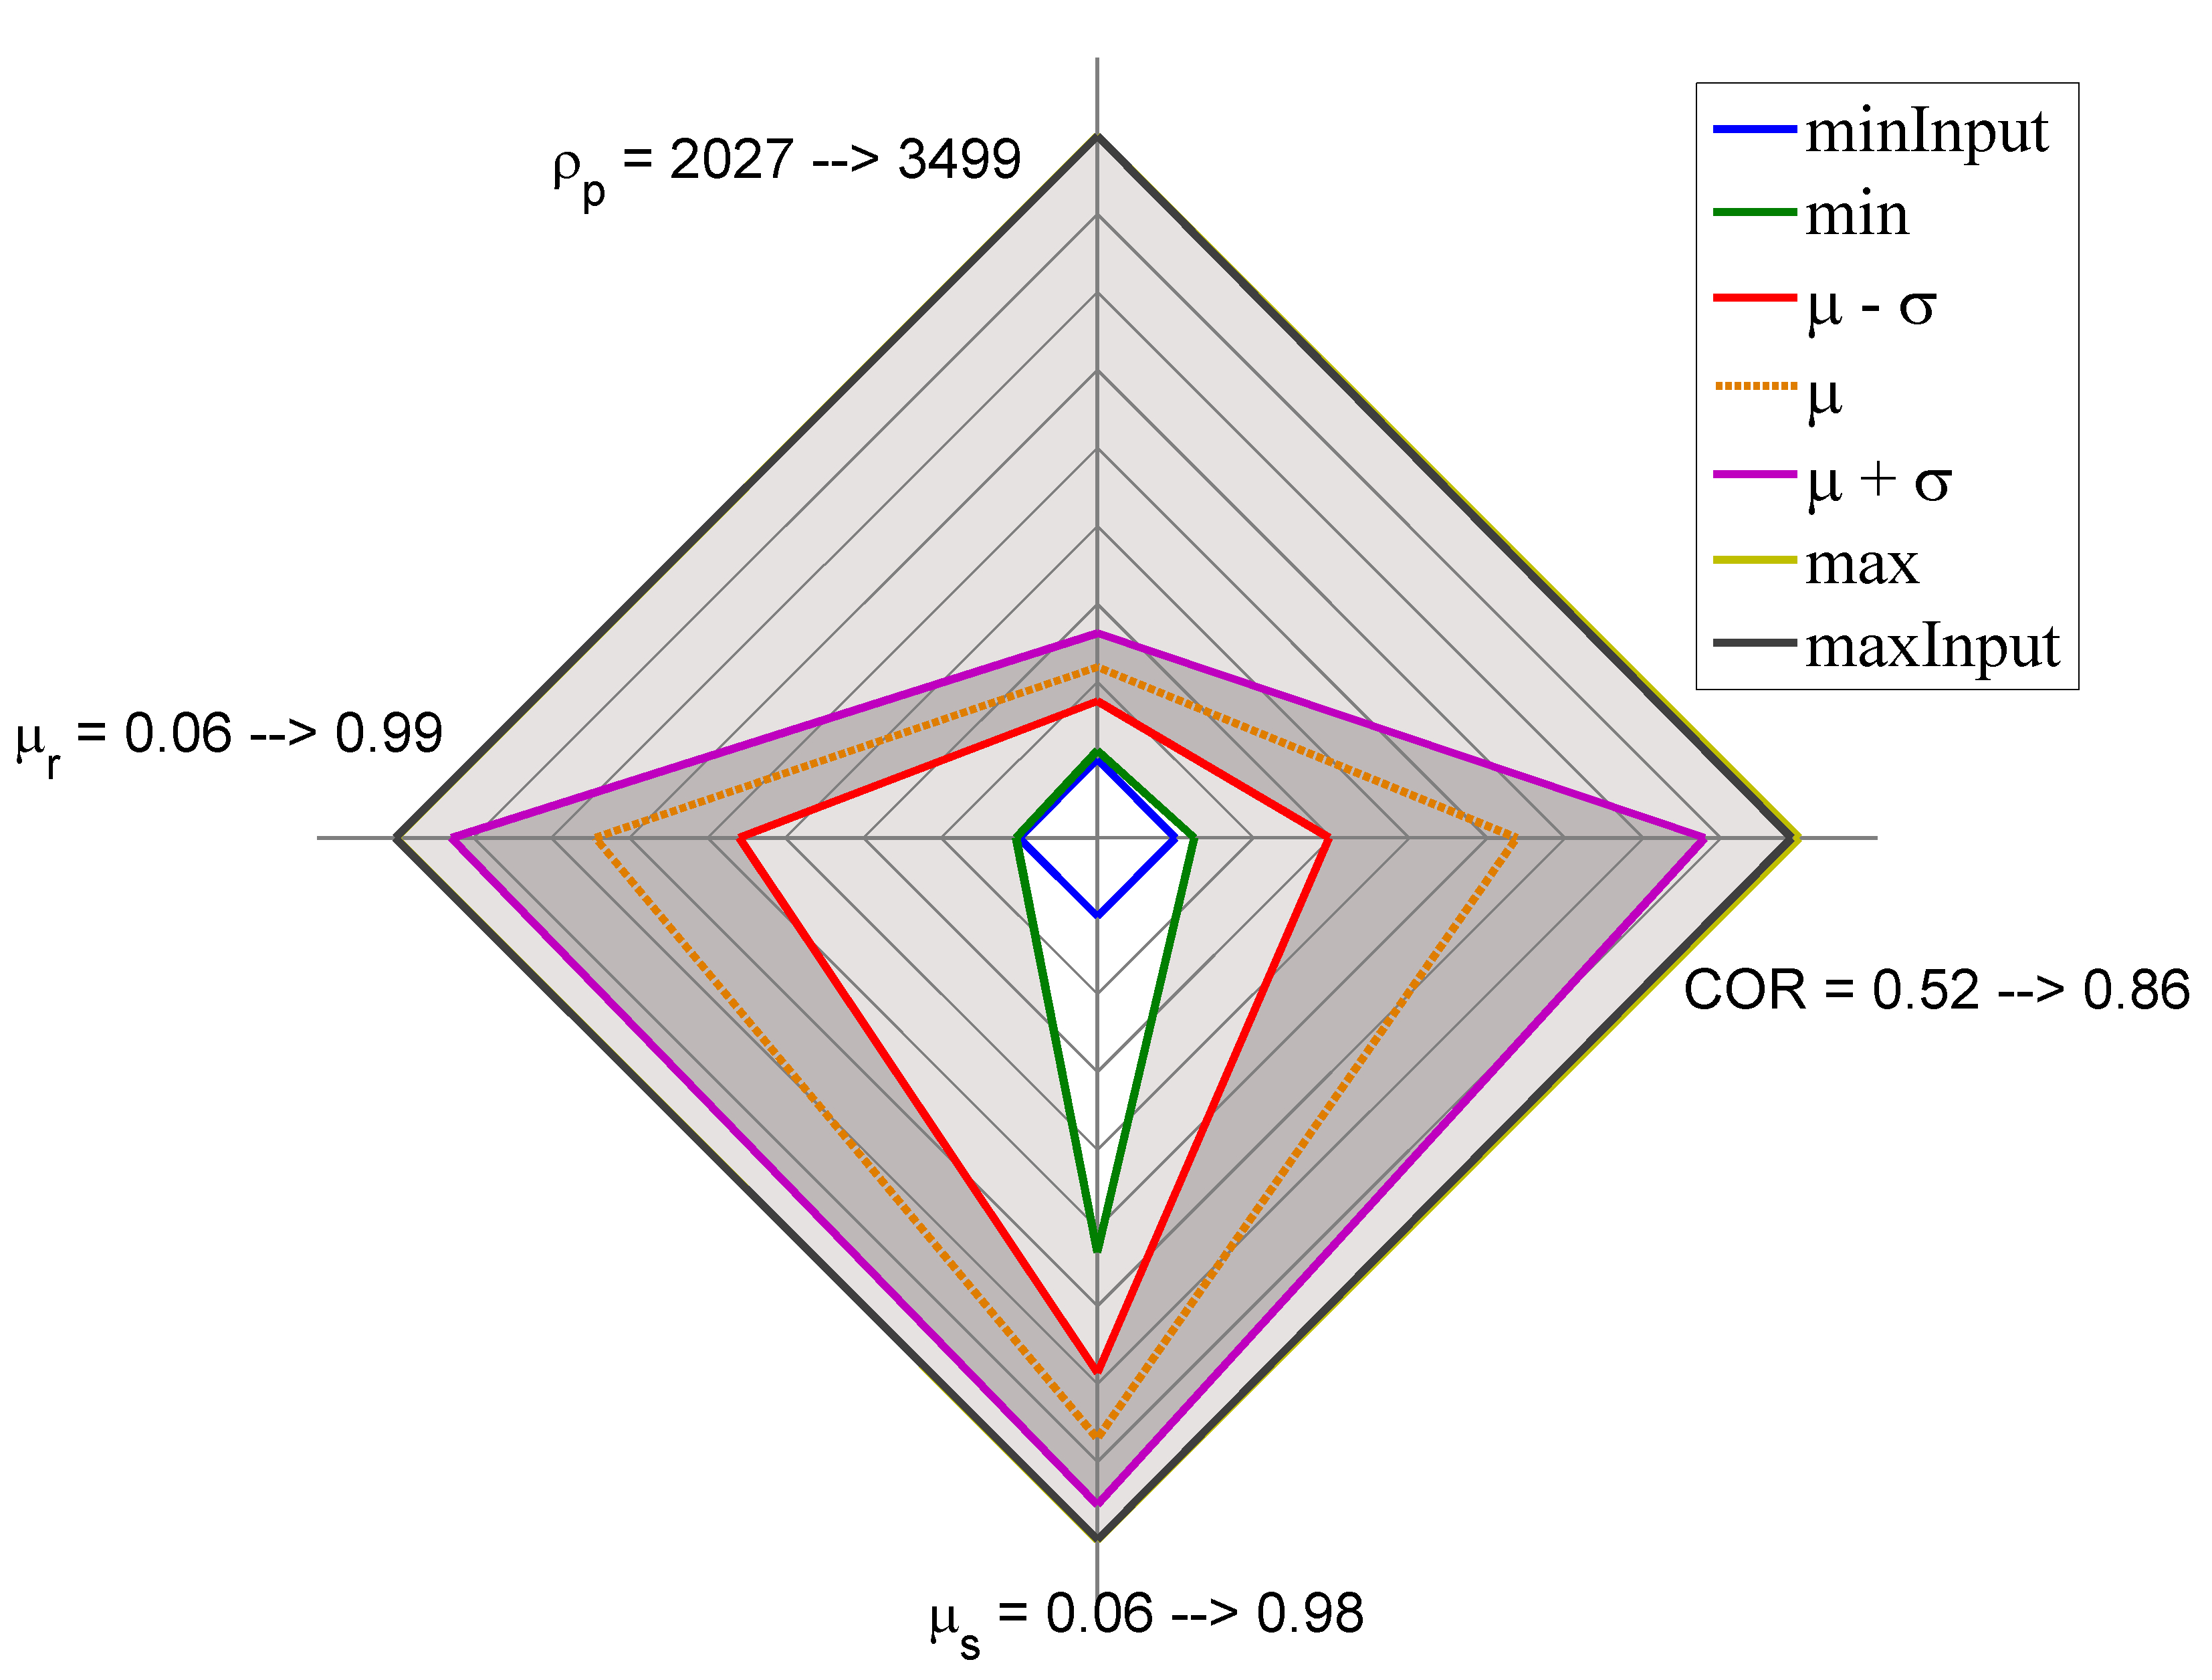
\includegraphics[width=\textwidth]{24radarpirker1schulze10070}
        \caption{Parameter space plot, $SSC$, $\sigma_n=10070$ Pa, P=1.0}
        \label{fig:24radarpirker1schulze10070}
    \end{subfigure} 
        \begin{subfigure}[b]{0.32\textwidth}
        %\includegraphics[width=.45\columnwidth]
        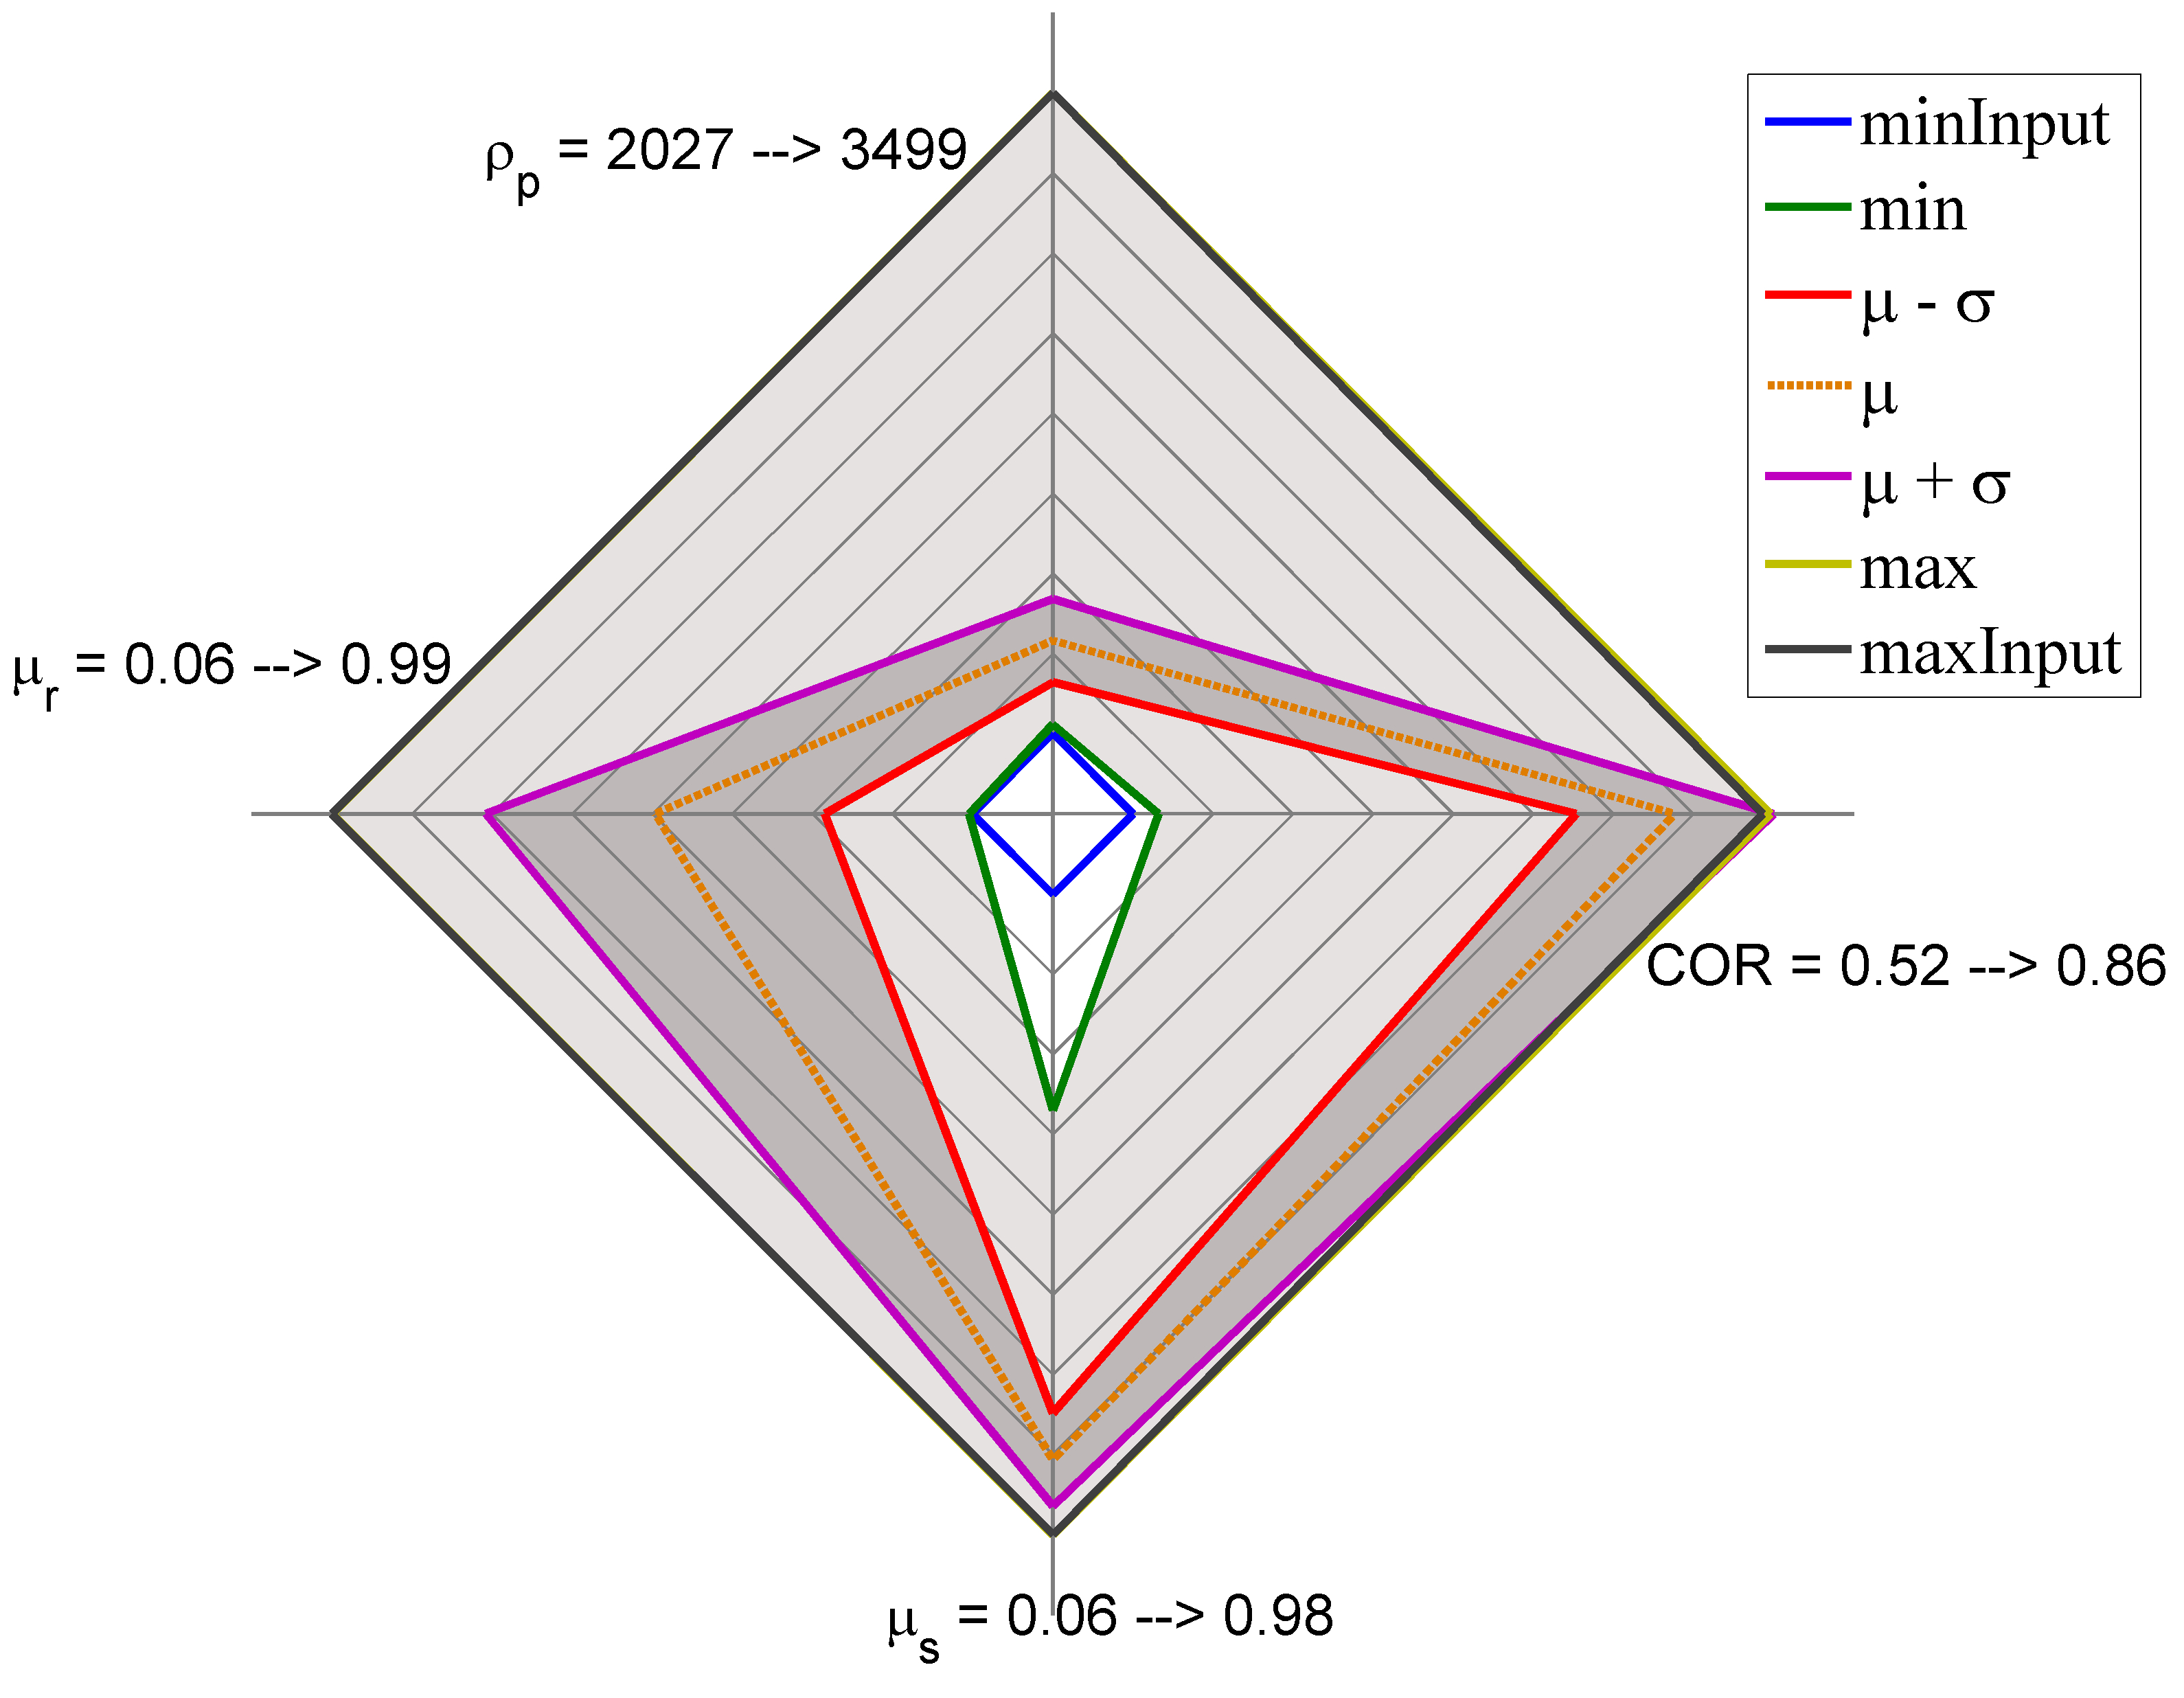
\includegraphics[width=\textwidth]{28radarpirker12schulze10070}
        \caption{Parameter space plot, $SSC$, $\sigma_n=10070$ Pa, P=1.2}
        \label{fig:28radarpirker12schulze10070} 
    \end{subfigure}
    \caption[Parameter space plot of valid simulations parameters for three different
    bulk behaviours measured by SSC]{\small{Parameter space plot of valid
    simulation parameters for three different bulk behaviours measured by a shear cell
    tester ($SSC$).
    Each axis of the parameter space plot represents one simulation parameter.
    The shaded area indicates valid parameter combinations, and dark shaded
    values indicate the confidence range.
	The marked combinations for $\sigma_n=10070$ Pa are presented.
    Further explanations can be found in
   Section \ref{subsec:experimentsparameteridentification}.
   }}
    \label{fig:29schulzeradarandcloud}
\end{figure}
%************************************************
\begin{figure}[htp] \centering

    \begin{subfigure}[b]{0.32\textwidth}
        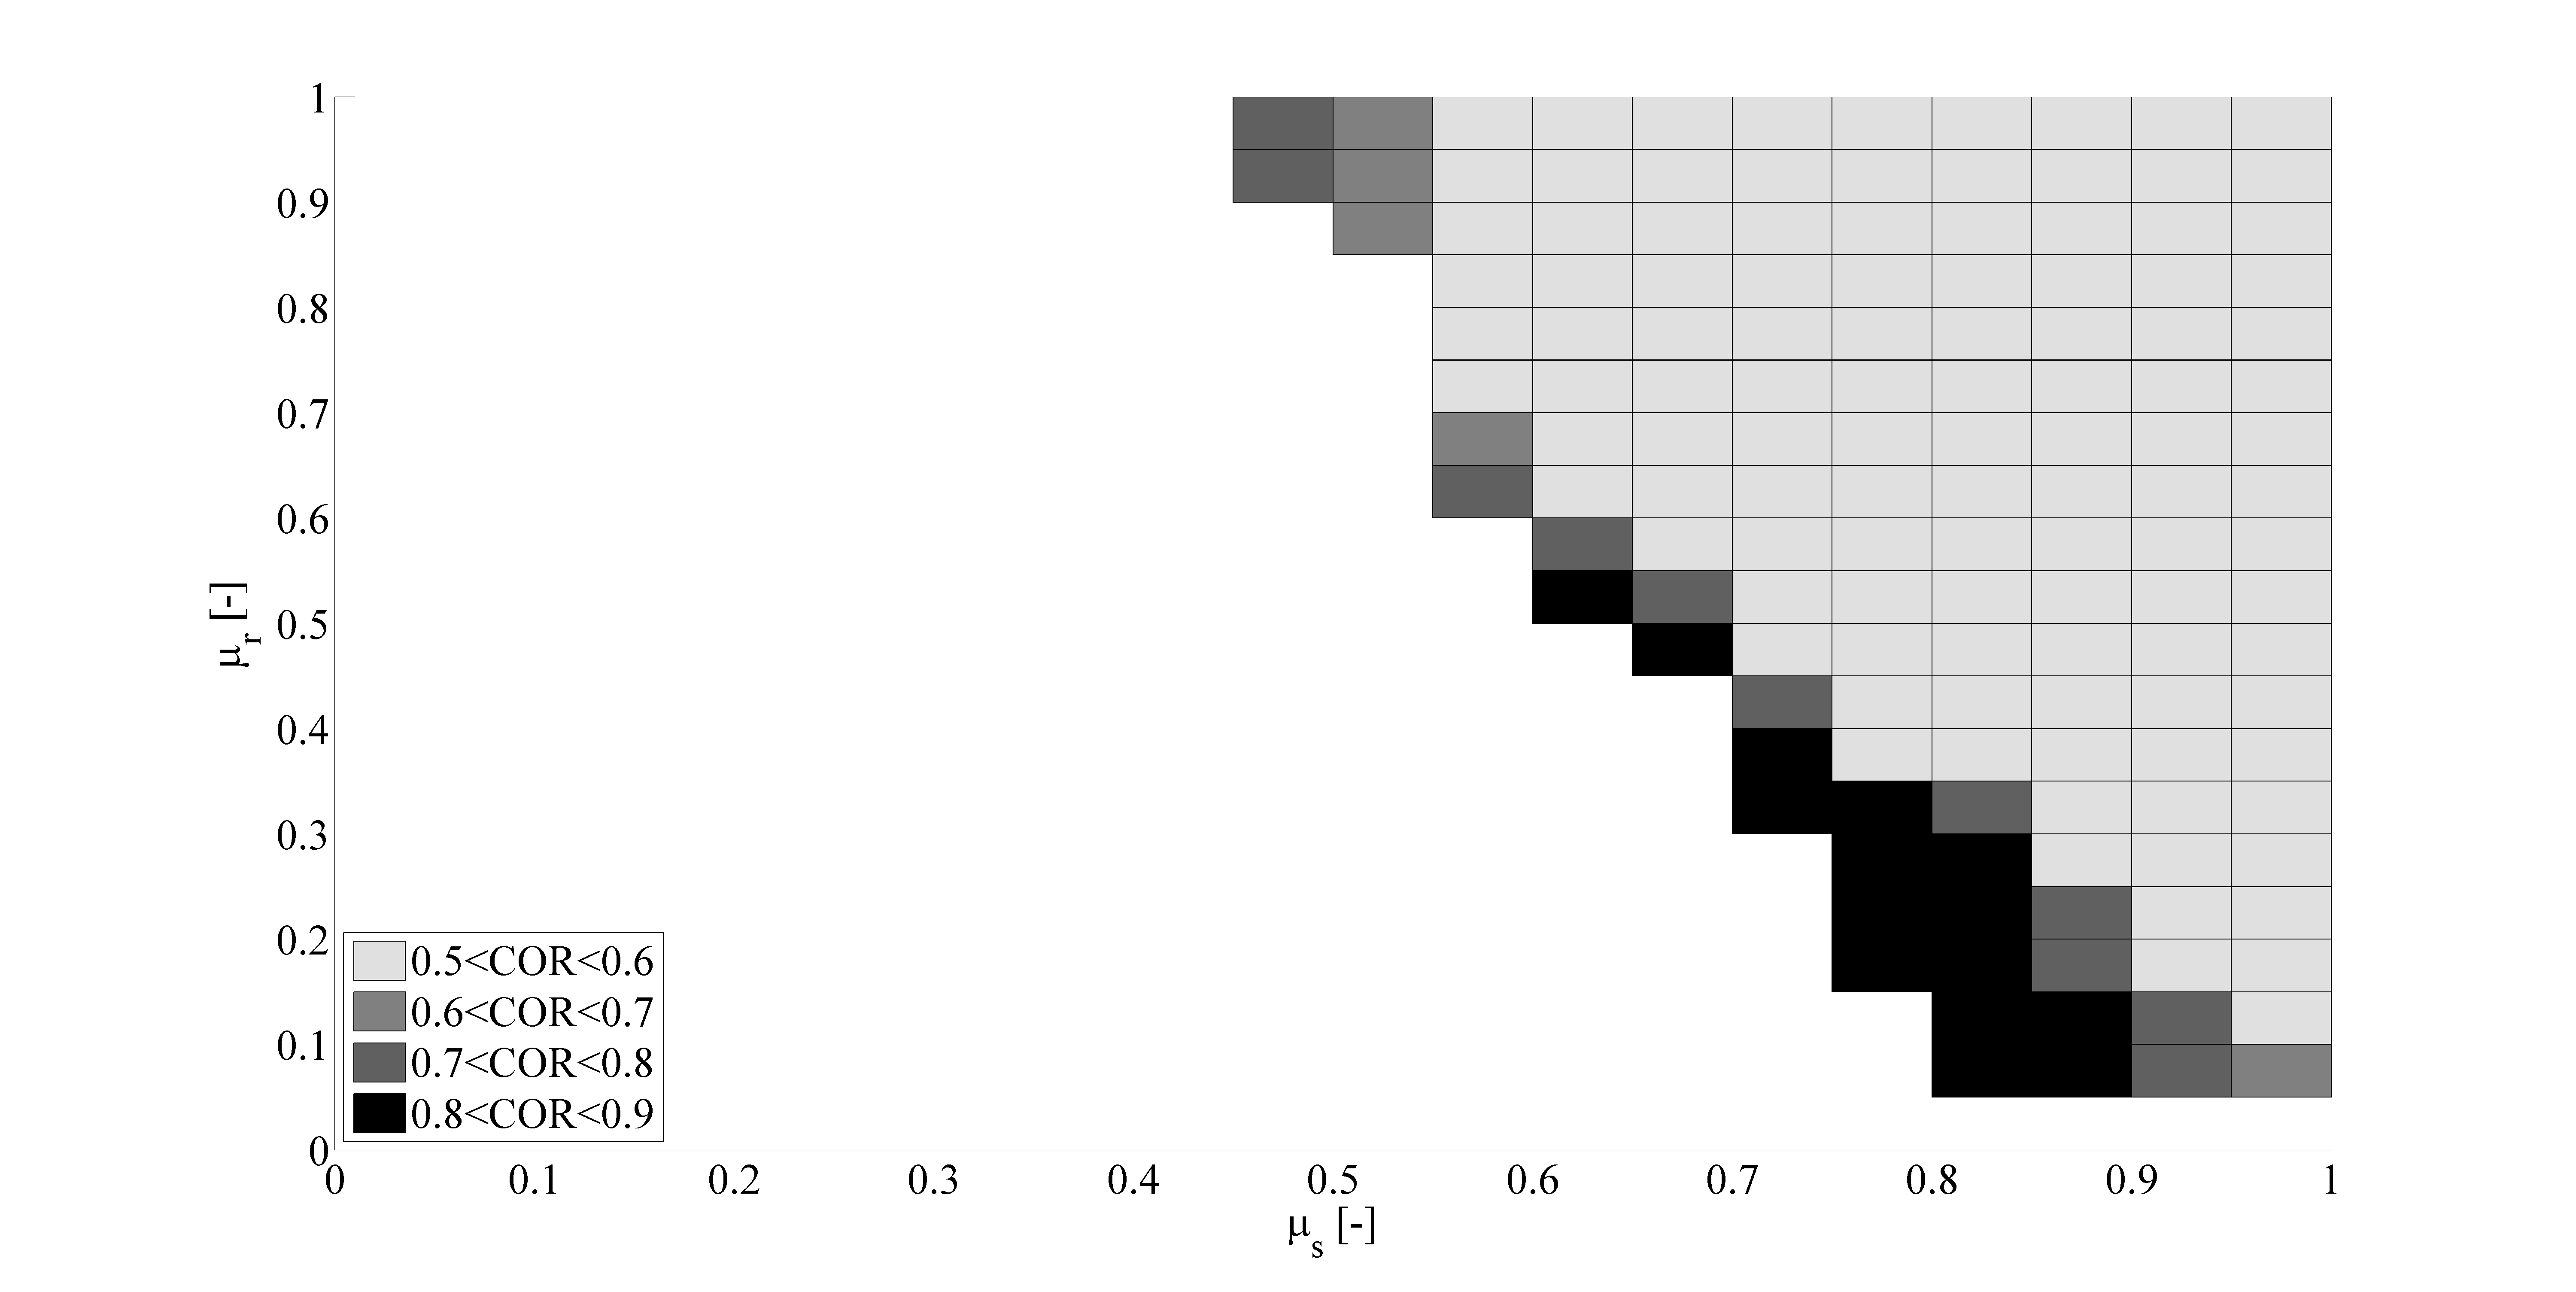
\includegraphics[width=\textwidth]{27cloudpirker08schulze10070}
        \caption{Density plot, $SSC$, $\sigma_n=10070$ Pa, P=0.8}
        \label{fig:27cloudpirker08schulze10070} 
    \end{subfigure}
    \begin{subfigure}[b]{0.32\textwidth}
        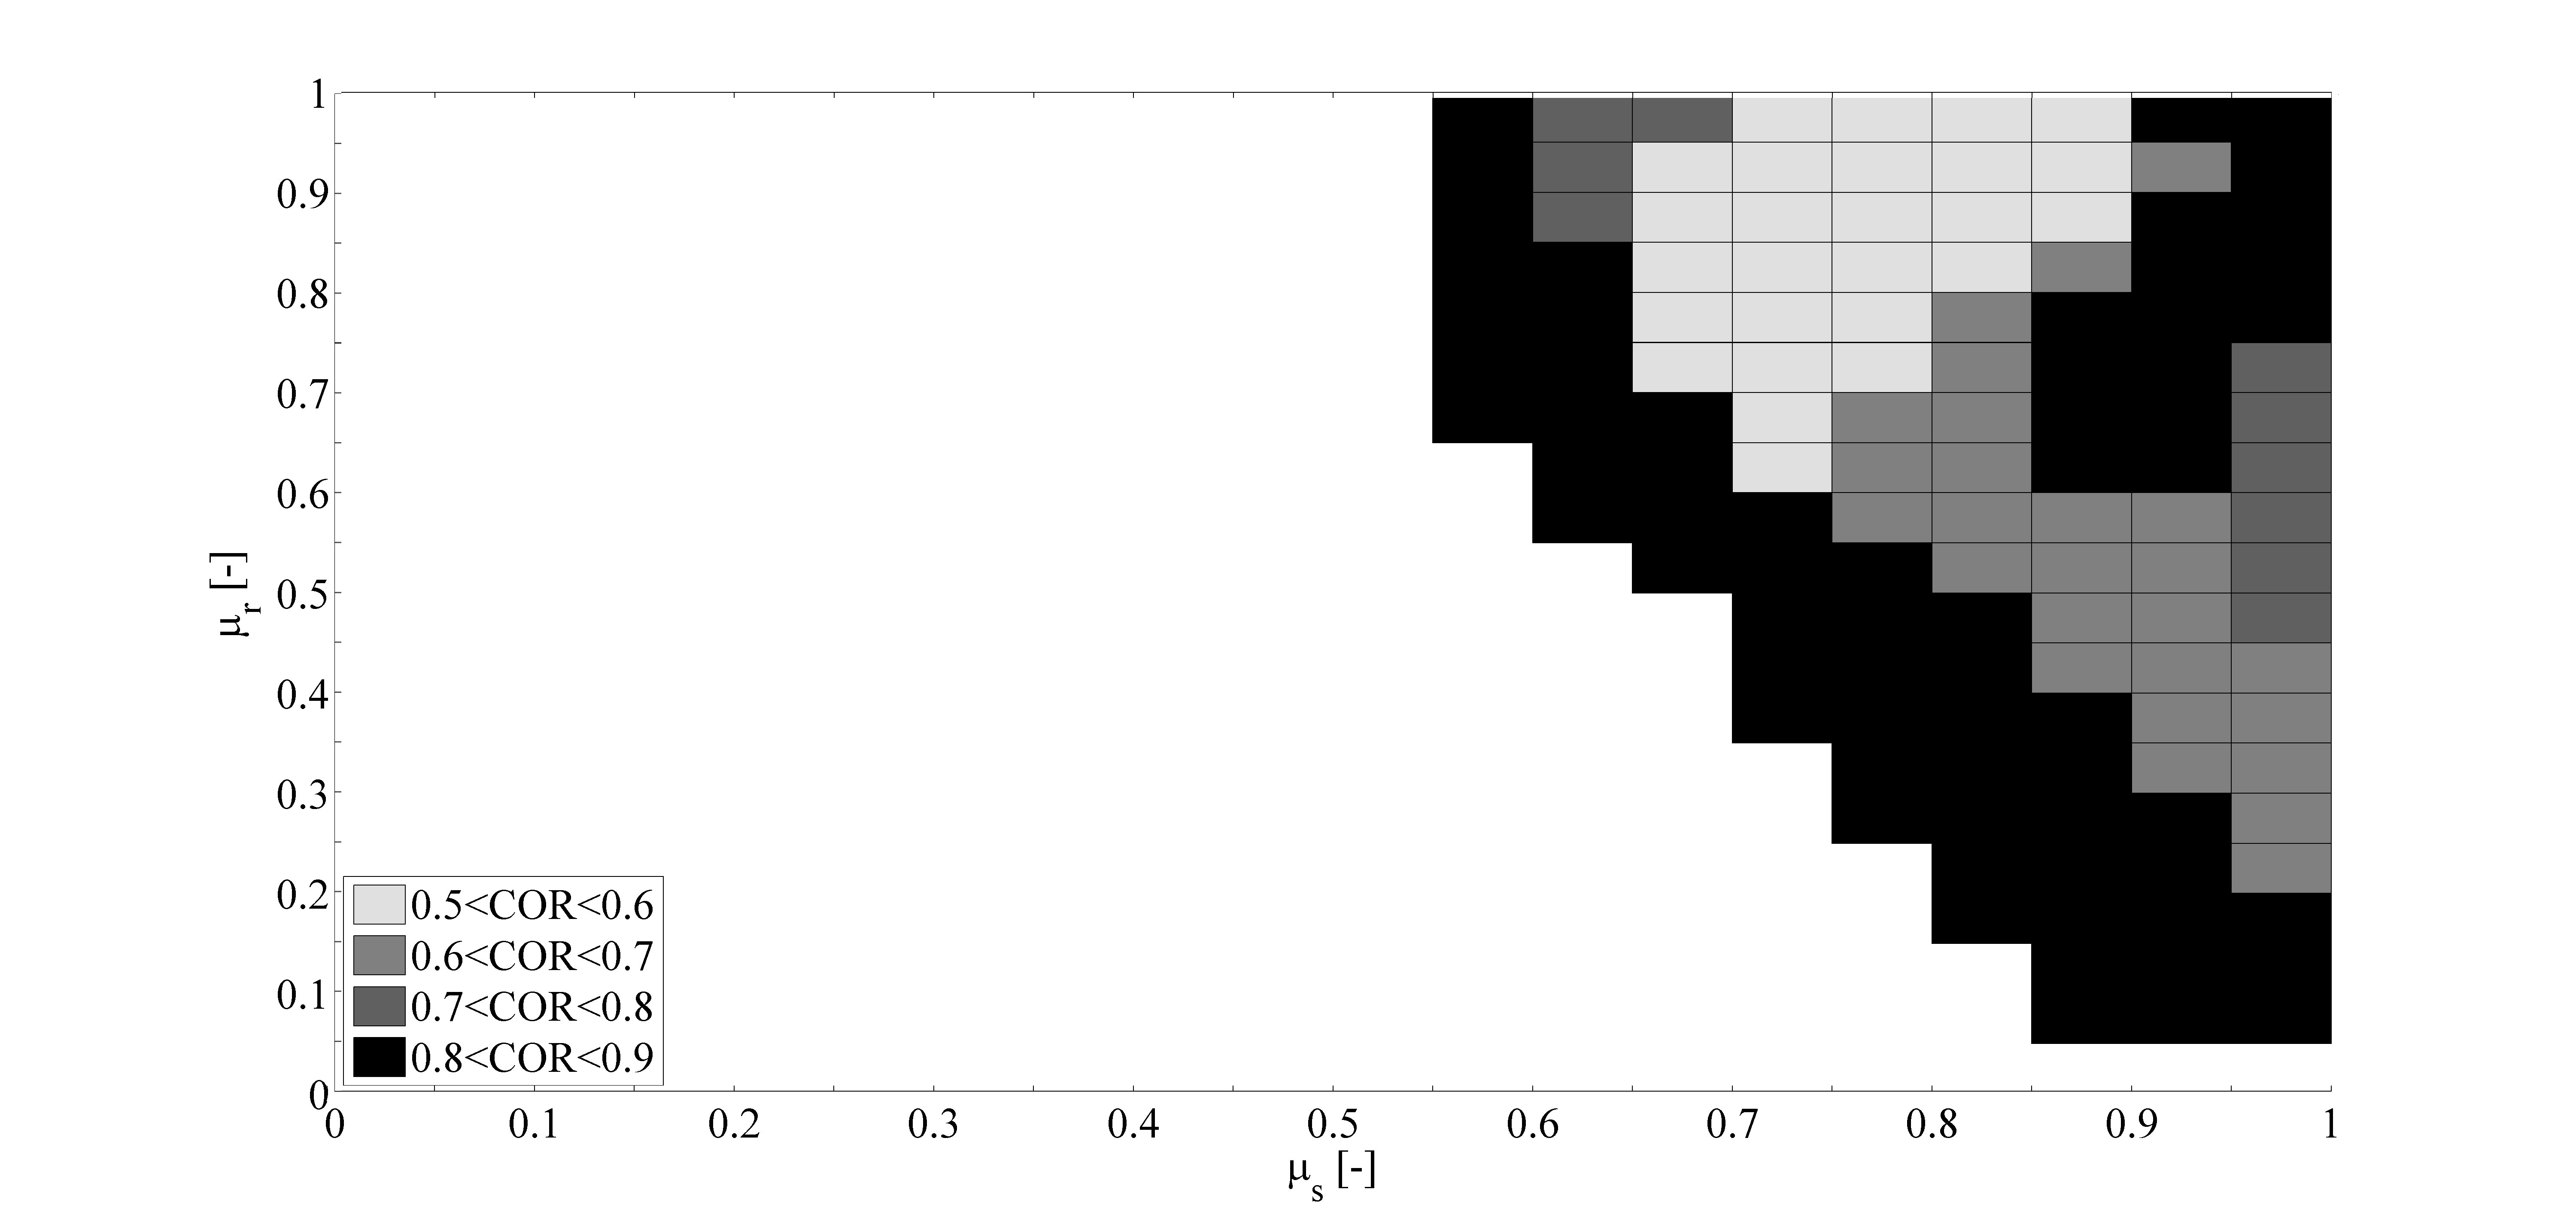
\includegraphics[width=\textwidth]{25cloudpirker1schulze10070}
        \caption{Density plot, $SSC$, $\sigma_n=10070$ Pa, P=1.0}
        \label{fig:25cloudpirker1schulze10070}
    \end{subfigure}
    \begin{subfigure}[b]{0.32\textwidth}
        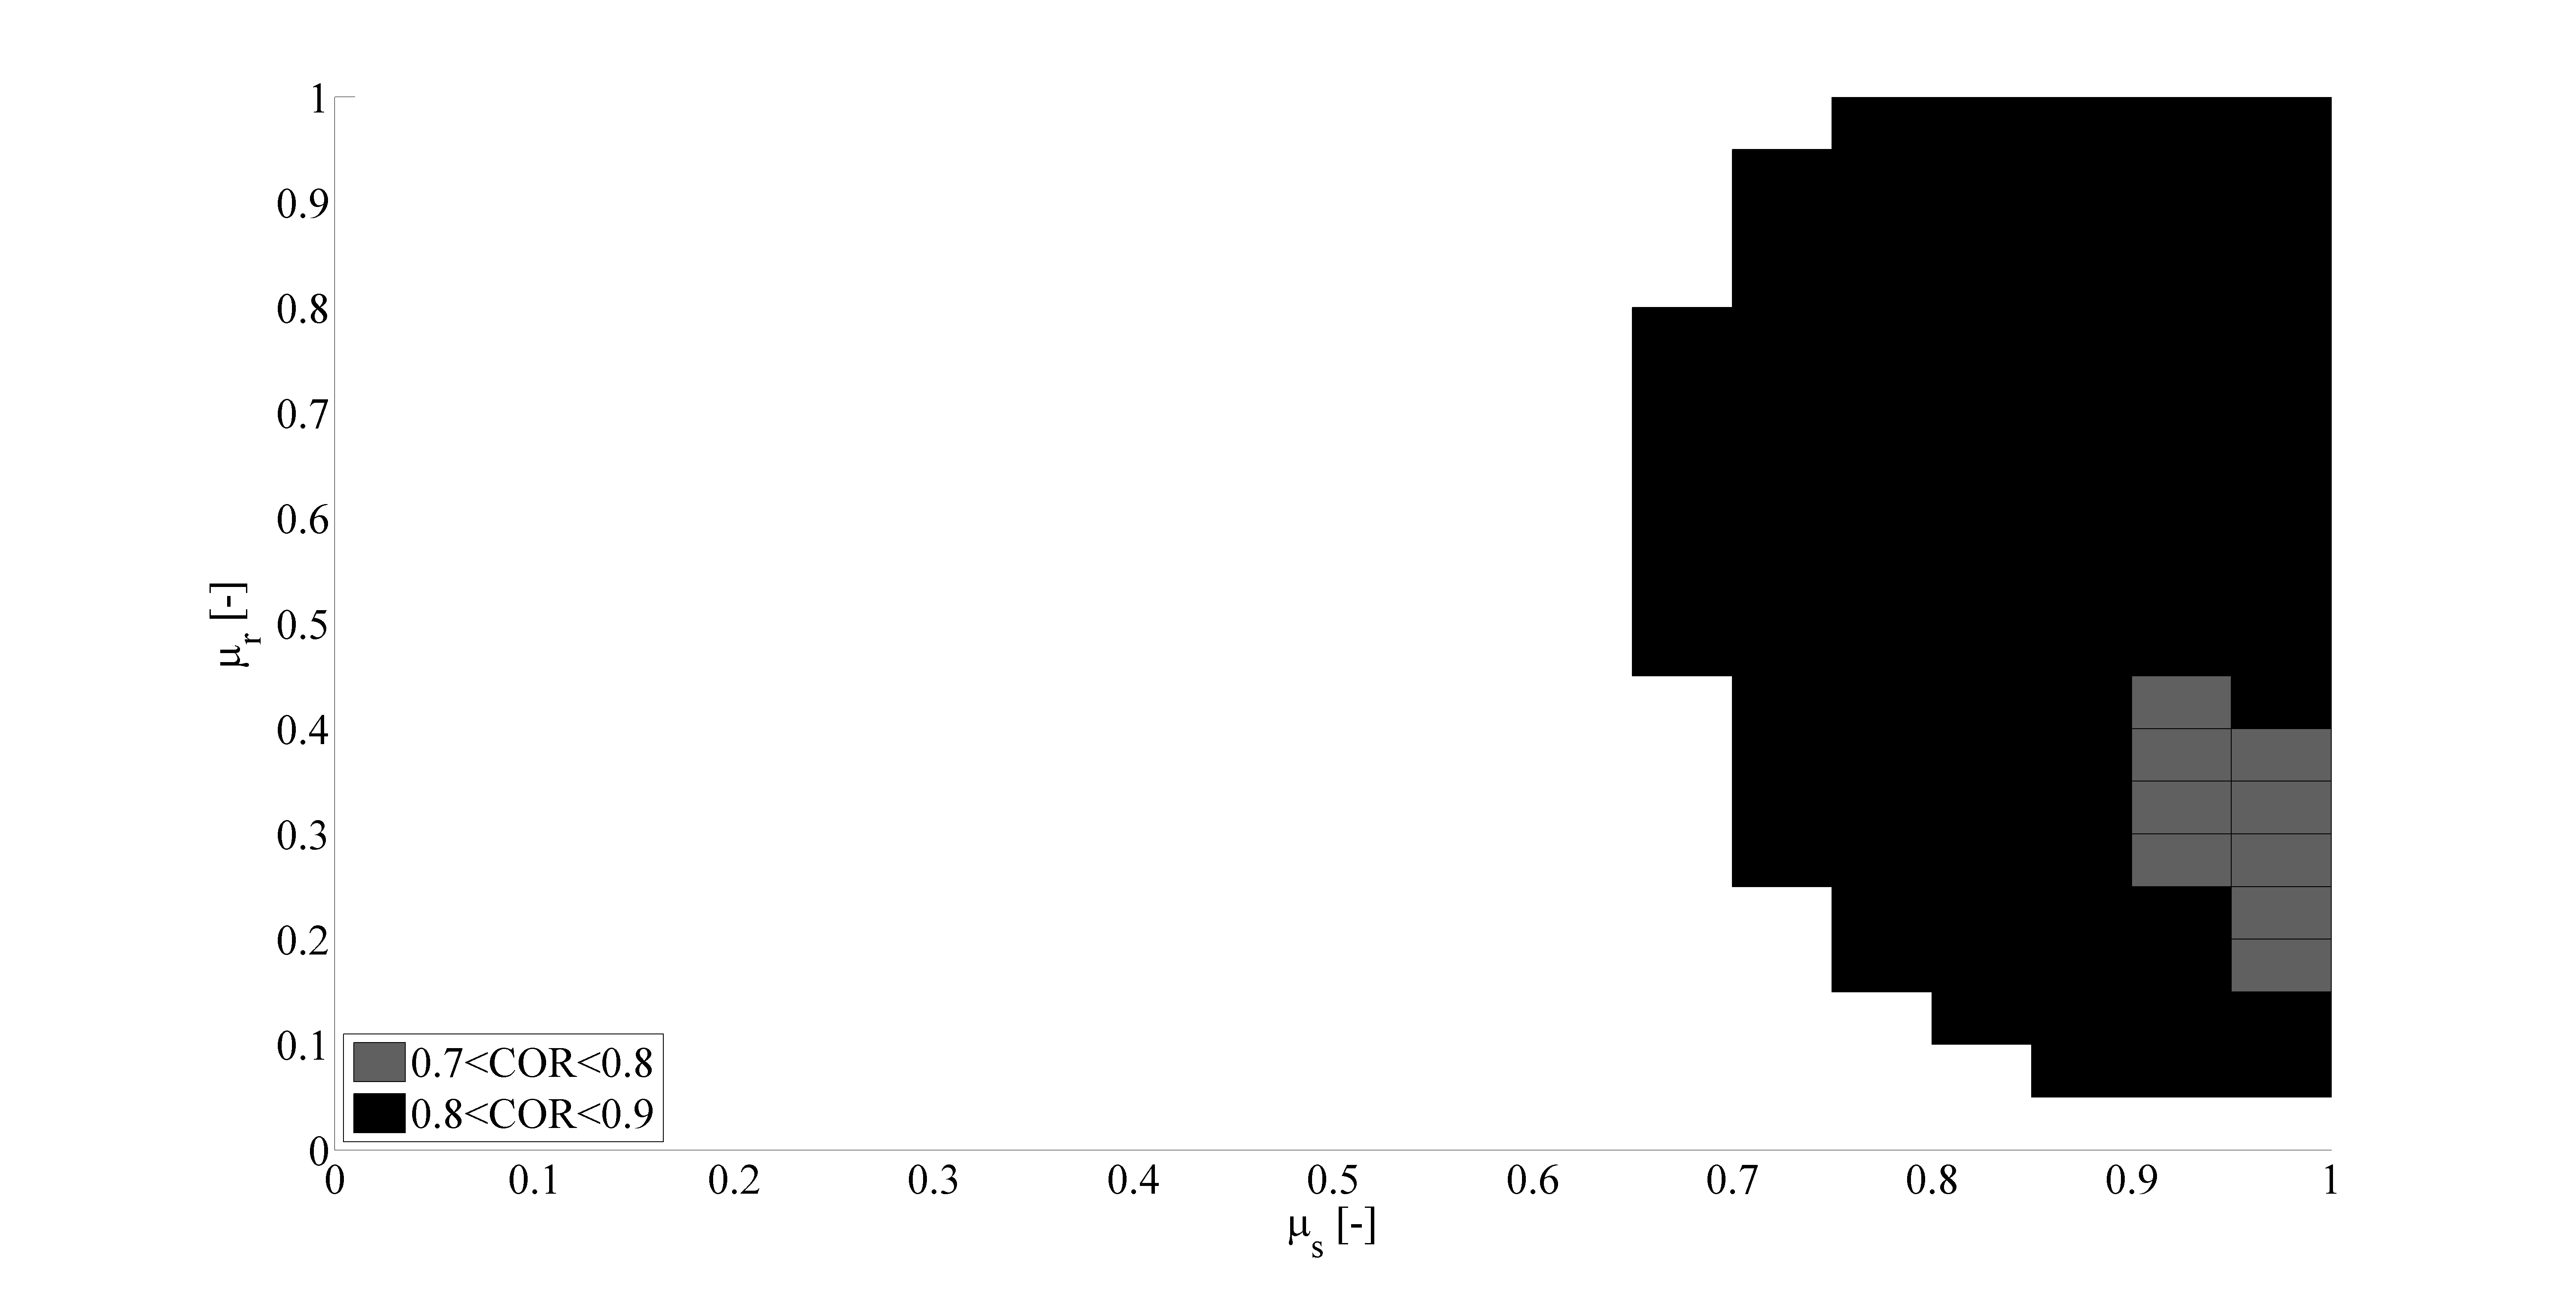
\includegraphics[width=\textwidth]{30cloudpirker12schulze10070}
        \caption{Density plot, $SSC$, $\sigma_n=10070$ Pa, P=1.2}
        \label{fig:30cloudpirker12schulze10070} 
    \end{subfigure}
    \caption[Density plot comparison of SSC results]{\small{Density plot
    comparison of shear cell tester ($SSC$) results. The marked combinations for
    $\sigma_n=10070 ~Pa$ are presented.
    Density plot of the particles' coefficient of restitution (COR) as a
    function of the coefficient of sliding friction ($\mu_s$) and the
    coefficient of rolling friction ($\mu_r$); 
    in the white area, no valid sets of simulation parameters can be found.
	In each cell the valid sets are grouped according to the 4 different COR
	ranges.
	Each cell is colored according to the group with the most members. 
    The values plotted here were initially
    selected between the numerical
    values from the Artificial Neural Network with the original
    experimental results for the $SSC$, with a product coefficient $P=1.0$ (Fig.
    \ref{fig:25cloudpirker1schulze10070}). 
    Subsequently, they were chosen with  
    a lower virtual shear stress ($P=0.8$)
    (\ref{fig:27cloudpirker08schulze10070}).
    The last image (Fig. \ref{fig:30cloudpirker12schulze10070}) represents
    the selection with a higher virtual shear stress ($P=1.2$).    }}
    \label{fig:29schulzeradarandcloud}
\end{figure}
%************************************************
\begin{figure}[htp] \centering
    \begin{subfigure}[b]{0.4\textwidth}
        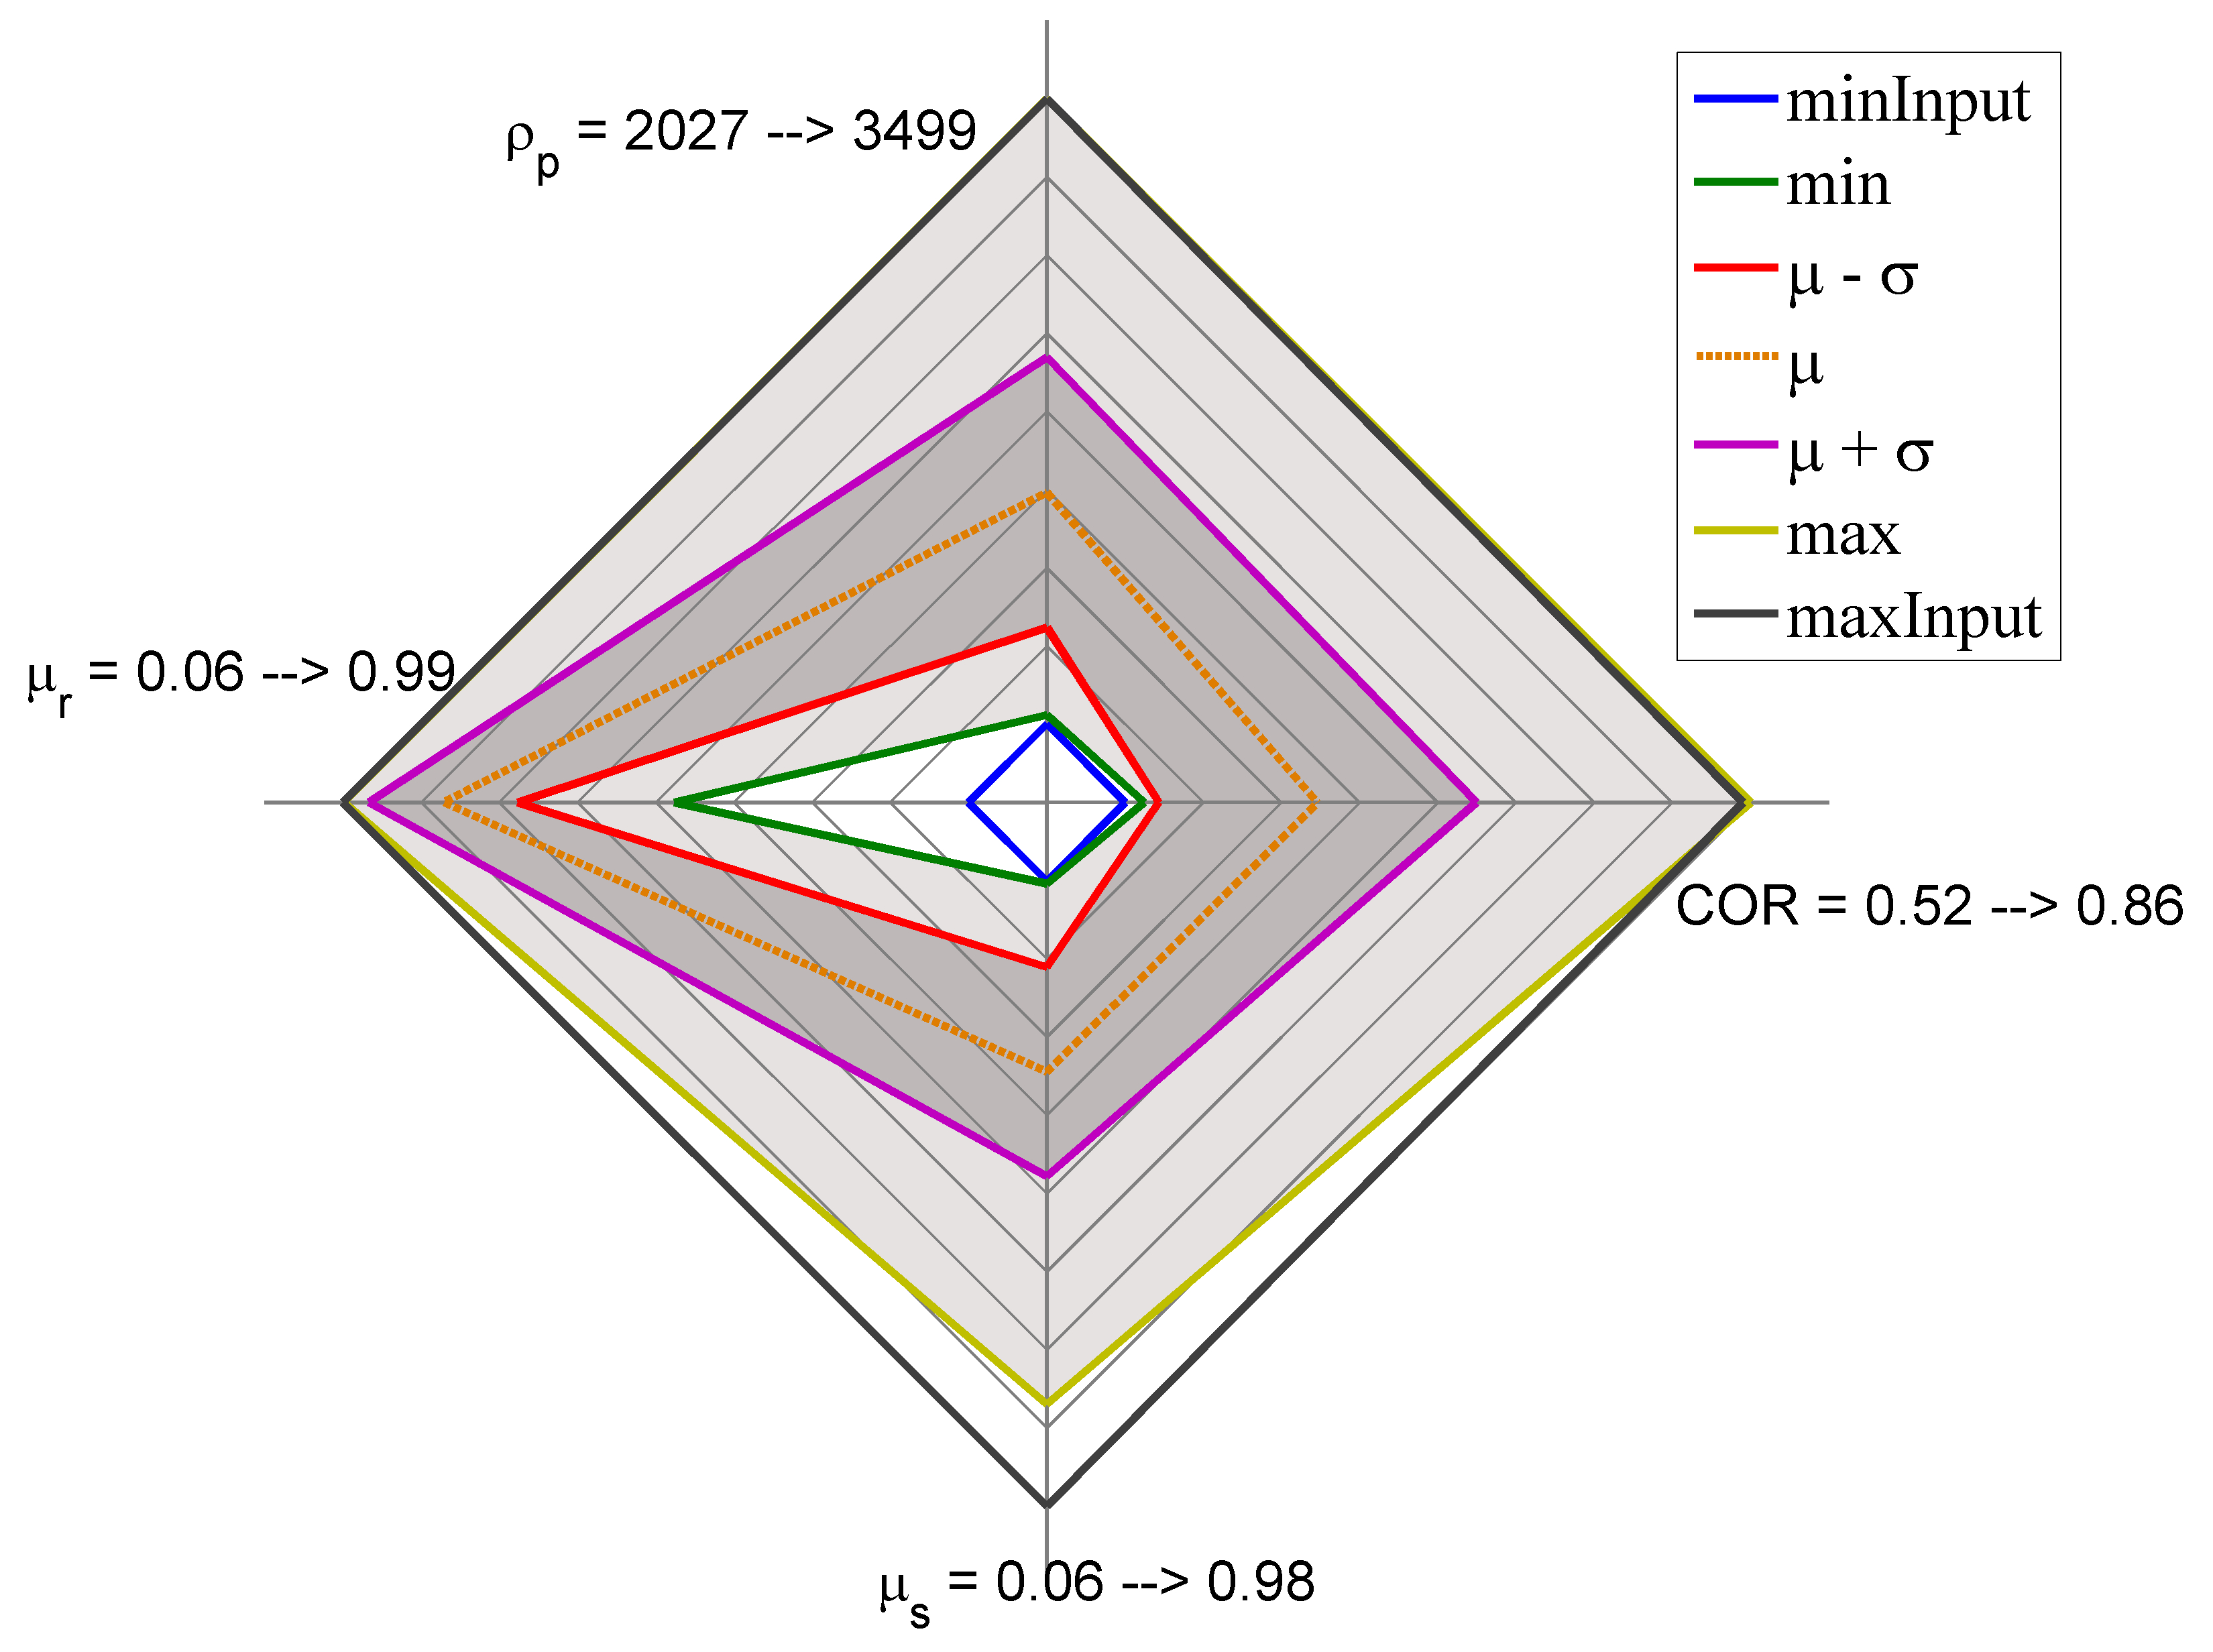
\includegraphics[width=\textwidth]{31radarpirker1aor}
        \caption{Parameter space plot, $AoR_{exp} = 38.85 ^\circ$}
        \label{fig:31radarpirker1aor} 
    \end{subfigure}
        \begin{subfigure}[b]{0.4\textwidth}
        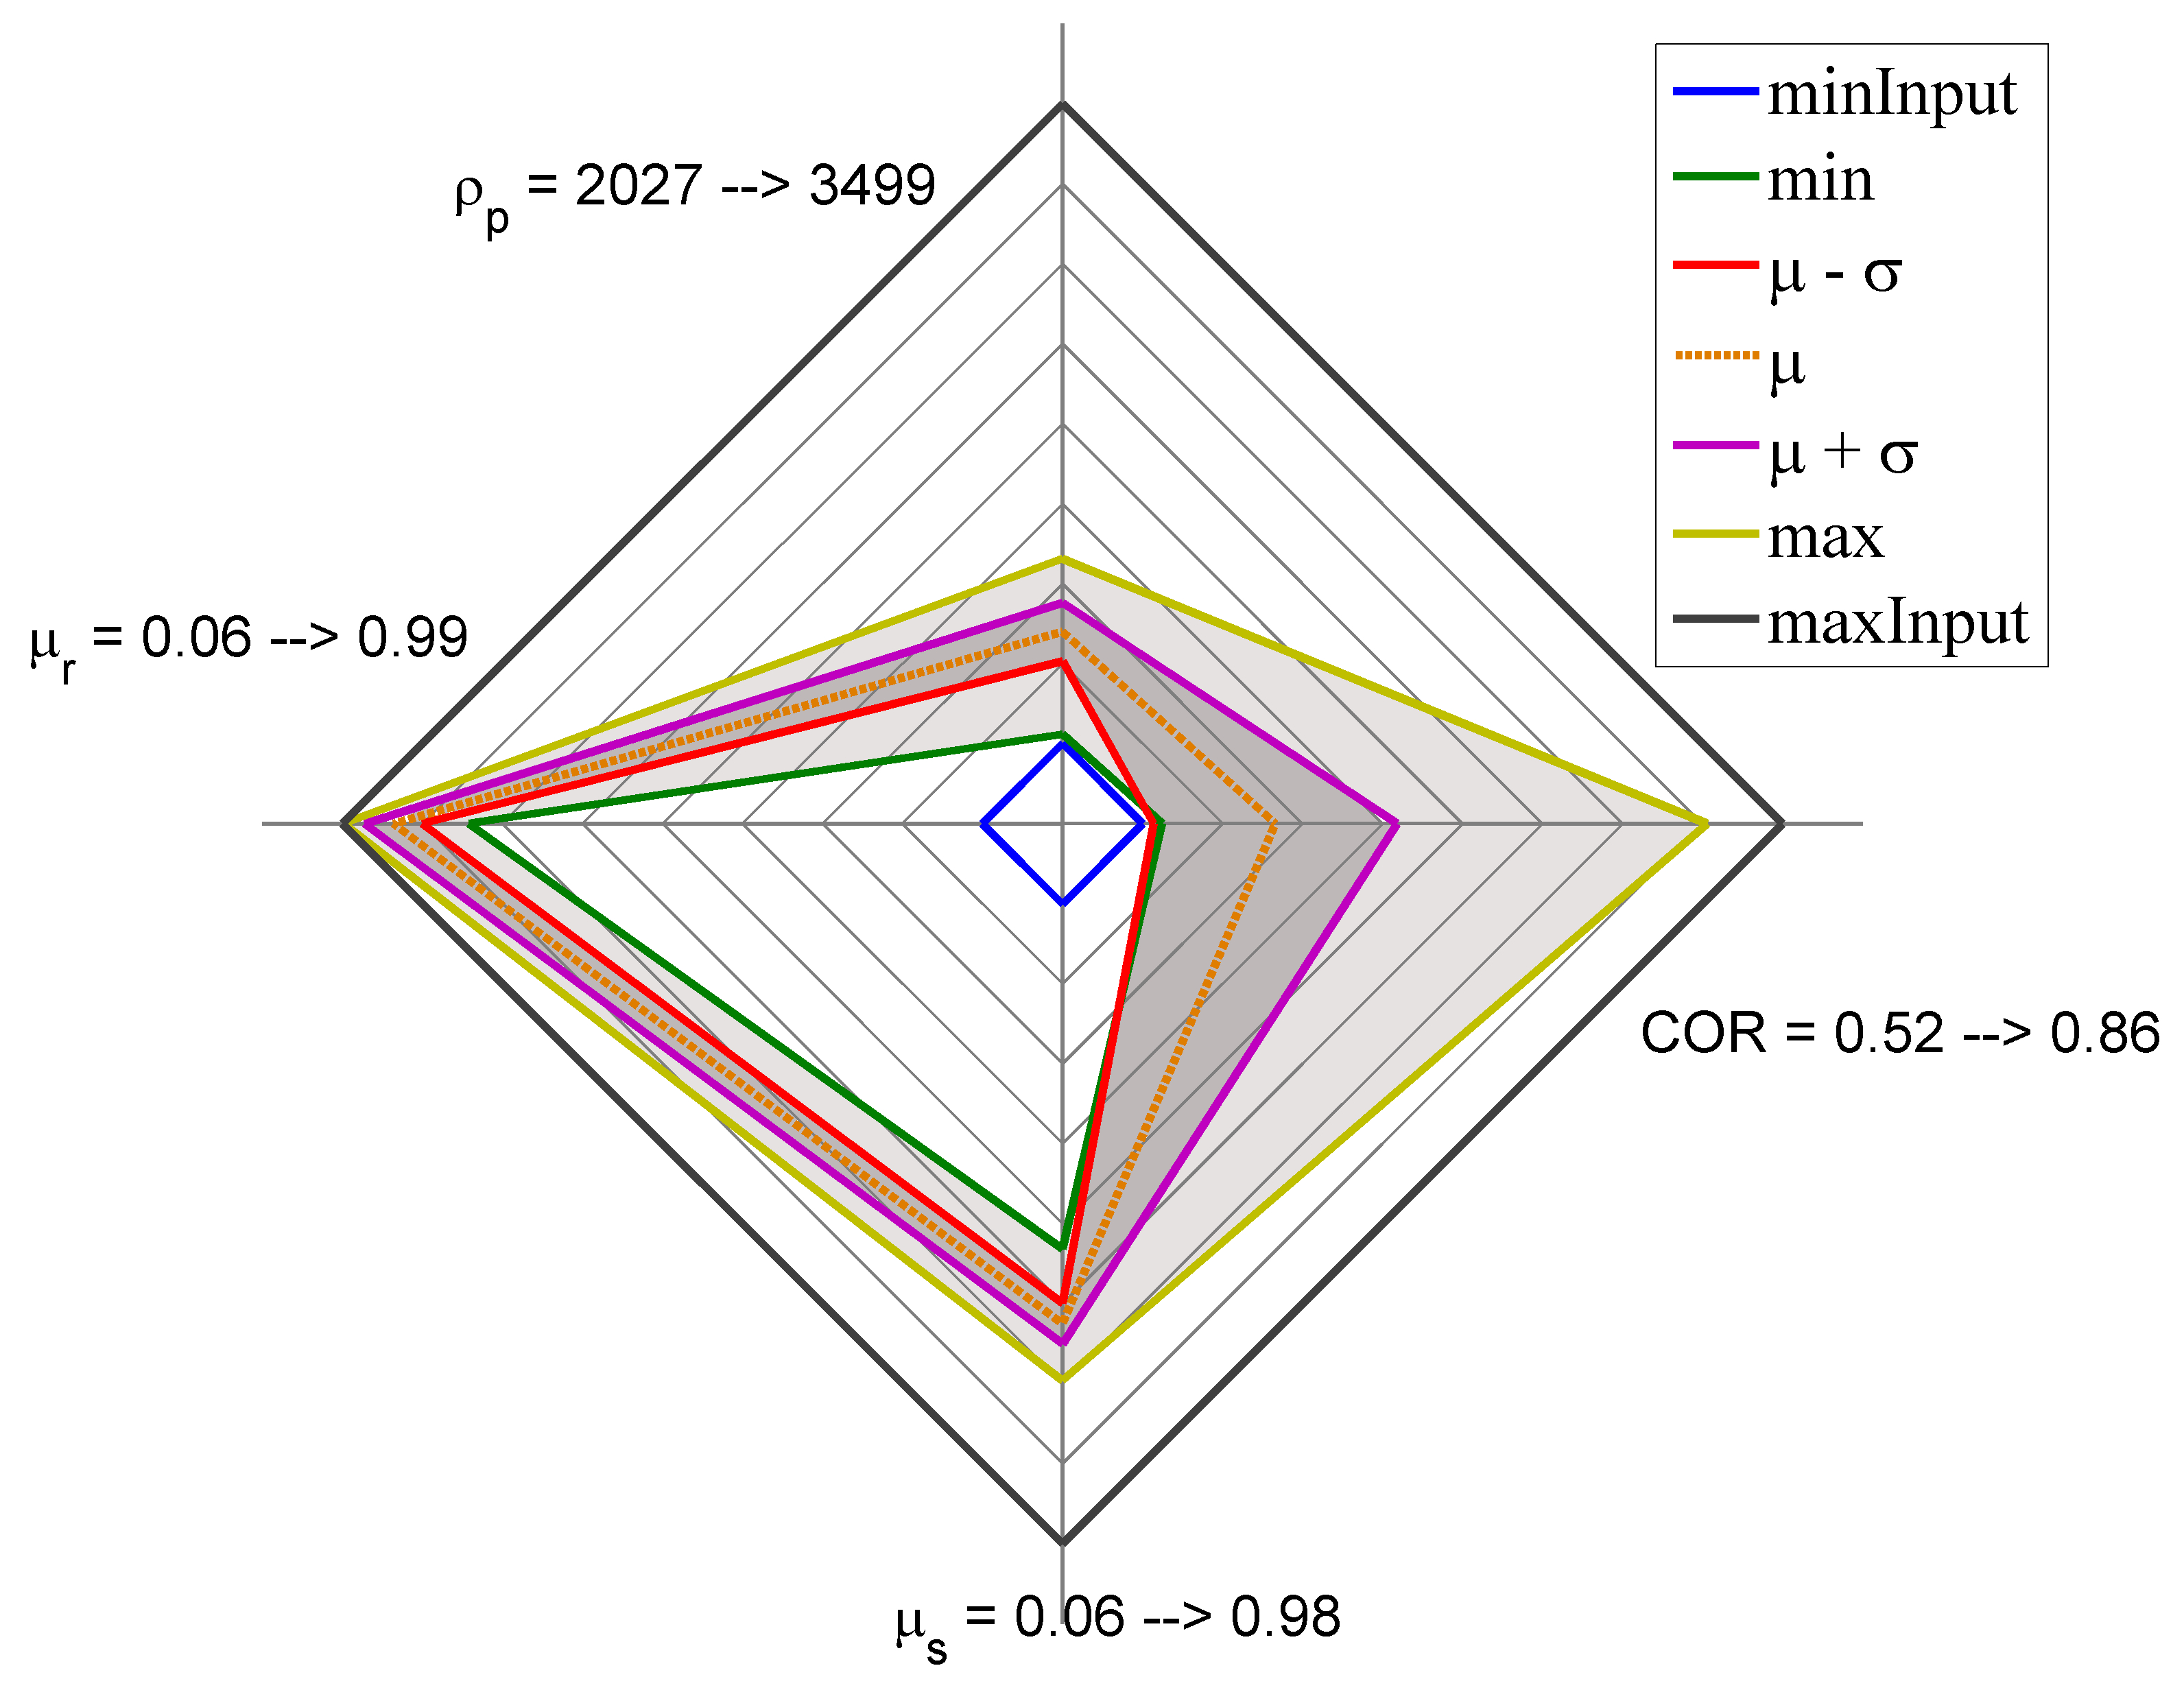
\includegraphics[width=\textwidth]{33radarpirker1schulze10070aor}
        \caption{Parameter space plot, $AoR_{exp} = 38.85
        ^\circ$ \& $SSC$: $\sigma_n=10070$ Pa}
        \label{fig:33radarpirker1schulze10070aor} 
    \end{subfigure}
    \caption[Parameter space plots of valid simulation parameters for the AoR
    and the combination of AoR and SSC valid parameters]{\small{Parameter space
    plots of valid simulation parameters for the angle of repose tester ($AoR$) and the
    combination of $AoR$ and shear cell tester ($SSC$).
    Each axis of the parameter space plot represents one simulation parameter.
    The shaded area 
    and dark shaded values indicate
    valid parameters combinations and
    the confidence interval, respectively.
    Further explanations are given in Section
    \ref{subsec:experimentsparameteridentification}.}}
    \label{fig:35schulze10070aorradarandcloud}
\end{figure}
%************************************************
%************************************************
\section{Conclusions}
\label{sec:conclusions}
%************************************************
We have presented a two-step method for $DEM$ simulation parameter
identification. In the first step, an artificial neural network is 
trained using dedicated $DEM$ simulations in order to predict bulk 
behaviours as function of a set of $DEM$ simulation parameters. 
In the second step, this artificial neural network is then used 
to predict the bulk behaviour of a huge number of additional $DEM$ parameter
sets.
The main findings of this study can be summarized as follows:
\begin{itemize}
  \item{An artificial neural network can be trained by a limited number of
  dedicated $DEM$ simulations.
  		The trained artificial neural network is then able to predict
  		granular bulk behaviour.}
  \item{This prediction of granular bulk behaviour is much more efficient
  		than computationally expensive $DEM$ simulations.
  		Thus, the macroscopic output associated with a huge number of parameter sets
  		can be studied.}
  \item{If the predictions of the artificial neural network are compared to a bulk experiment, 
  		valid sets of $DEM$ simulation parameters can be readily deduced for a
  		specific granular material.}
  \item{This $DEM$ parameter identification method can be applied to
  arbitrary bulk experiments.
  		Combining two artificial neural networks which predict two different bulk
  		behaviours leads to winnowing the set of valid $DEM$ simulation parameters.}
\end{itemize}
As part of future work, we will develop this method further by considering
different fractions of granular materials, which will lead to size-dependent sets of $DEM$
simulation parameters.

%************************************************
%************************************************

\section*{Acknowledgments}\label{sec:Acknowledgments}

This study was funded by the Christian Doppler Forschungsgesellschaft, Siemens
VAI Metals Technologies, and Voestalpine Stahl. The authors gratefully
aknowledge their support.

%************************************************

% % %\begin{thebibliography}{10}
% \bibliographystyle{splncs}
% \bibliography{Bibliografia}
% 
% %\end{thebibliography}
%************************************************
\begin{thebibliography}{10}
\expandafter\ifx\csname url\endcsname\relax
  \def\url#1{\texttt{#1}}\fi
\expandafter\ifx\csname urlprefix\endcsname\relax\def\urlprefix{URL }\fi
\expandafter\ifx\csname href\endcsname\relax
  \def\href#1#2{#2} \def\path#1{#1}\fi

\bibitem{RefWorks:130}
P.~W. Cleary, M.~L. Sawley, DEM modelling of industrial granular flows: 3D case
  studies and the effect of particle shape on hopper discharge, Applied
  Mathematical Modelling 26~(2) (2002) 89--111.

\bibitem{RefWorks:172}
P.~A. Cundall, O.~D.~L. Strack, A discrete numerical model for granular
  assemblies, Geotechnique 29~(Volume 29, Issue 1) (1979) 47--65(18).

\bibitem{RefWorks:148}
L.~Vu-Quoc, X.~Zhang, An accurate and efficient tangential force-displacement
  model for elastic frictional contact in particle-flow simulations, Mechanics
  of Materials 31~(4) (1999) 235--269.

\bibitem{RefWorks:145}
A.~D. Renzo, F.~P.~D. Maio, Comparison of contactforce models for the
  simulation of collisions in DEM-based granular flow codes, Chemical
  Engineering Science 59~(3) (2004) 525--541.

\bibitem{RefWorks:87}
C.~M. Wensrich, A.~Katterfeld, Rolling friction as a technique for modelling
  particle shape in DEM, Powder Technology 217~(0) (2012) 409--417.

\bibitem{RefWorks:136}
C.~Kloss, C.~Goniva, A.~Hager, S.~Amberger, S.~Pirker, Models, algorithms and
  validation for opensource DEM and CFDDEM, Progress in Computational Fluid
  Dynamics, an International Journal 12~(2) (2012) 140--152.

\bibitem{RefWorks:139}
A.~Aigner, S.~Schneiderbauer, C.~Kloss, S.~Pirker, Determining the coefficient
  of friction by shear tester simulation, 3rd International Conference on
  Particle-Based Methods (2013) 335--342.

\bibitem{RefWorks:86}
D.~Hohner, S.~Wirtz, V.~Scherer, A numerical study on the influence of particle
  shape on hopper discharge within the polyhedral and multi-sphere discrete
  element method, Powder Technology 226~(0) (2012) 16--28.

\bibitem{RefWorks:131}
J.~Ai, J.-F. Chen, J.~M. Rotter, J.~Y. Ooi, Assessment of rolling resistance
  models in discrete element simulations, Powder Technology 206~(3) (2011)
  269--282.

\bibitem{RefWorks:177}
M.~Combarros, H.~J. Feise, H.~Zetzener, A.~Kwade, Segregation of particulate
  solids: Experiments and DEM simulations, Particuology 12~(0) (2014) 25--32.

\bibitem{RefWorks:91}
A.~Alenzi, M.~Marinack, C.~F. Higgs, J.~J. McCarthy, DEM validation using an
  annular shear cell, Powder Technology 248~(0) (2013) 131--142.

\bibitem{RefWorks:150}
B.~Vaferi, F.~Samimi, E.~Pakgohar, D.~Mowla, Artificial neural network approach
  for prediction of thermal behavior of nanofluids flowing through circular
  tubes, Powder Technology 267~(0) (2014) 1--10.

\bibitem{RefWorks:158}
S.~Haykin, Neural Networks and Learning Machines, no. v. 10, Prentice Hall,
  2009, 2008034079.

\bibitem{RefWorks:175}
N.~Tsafnat, N.~Amanat, A.~S. Jones, Analysis of coke under compressive loading:
  A combined approach using microcomputed tomography, finite element analysis,
  and empirical models of porous structures, Fuel 90~(1) (2011) 384--388.

\bibitem{RefWorks:176}
J.~Kovacik, Correlation between young modulus and porosity in porous materials,
  Journal of Material Science 18 (1999) 1007--1010.

\bibitem{RefWorks:143}
M.~J. Jiang, H.~S. Yu, D.~Harris, A novel discrete model for granular material
  incorporating rolling resistance, Computers and Geotechnics 32~(5) (2005)
  340--357.

\bibitem{RefWorks:160}
W.~L. Oberkampf, C.~J. Roy, Verification and Validation in Scientific
  Computing, Cambridge University Press, 2010.

\bibitem{RefWorks:180}
L.~Benvenuti, C.~Kloss, S.~Pirker, Identification of dem simulation parameters
  by artificial neural networks and bulk experiments, manuscript sumbitted for
  publication.

\end{thebibliography}

%************************************************


\end{document}


